\documentclass{jknotes}
\usepackage{joshkirklin}

\begin{document}

\institution{Cambridge Part III Maths}
\title{Black Holes}
\lecturer{Harvey Reall}
\notetaker{Josh Kirklin}
\date{Lent 2016}

\maketitle
\suggestionsspiel
In this course we take \(G=c=1\) and \(\Lambda=0\).
\tableofcontents

\section{Spherical stars}
\lecture{15/01/16}
Consider a gas of cold fermions. This gas will resist compression due to \emph{degeneracy pressure} resulting from the Pauli principle. For example, in a white dwarf star, gravity is balanced by electron degeneracy pressure. Using Newtonian gravity, we can find an upper limit on the mass of a stable white dwarf, known as the \emph{Chandrasekhar limit}:
\begin{equation}
    M_{\text{WD}} \lesssim 1.4M_{\astrosun}
\end{equation}

In a neutron star, gravity is balanced by neutron degeneracy pressure. Neutron stars are tiny; a neutron star with the mass of the sun has a radius of approximately \SI{10}{\kilo\meter} (for comparison, the sun has a radius of \(R_{\astrosun}\approx\SI{7e5}{\kilo\meter}\). At the surface of a neutron star, the gravitational potential \(|\phi|\approx0.1\). Recall that in order to be able to apply Newtonian gravity, we must have \(|\phi|\ll1\). \(0.1
\not\ll1\), so it is important to consider general relativity when reasoning about neutron stars.

In this section we will establish that \(M \lesssim 3M_{\astrosun}\) for \emph{any} cold star.

\subsection{Spherical symmetry and time independence}

Consider the round metric on \(S^2\):
\begin{equation}
    \dd{\Omega}^2 = \dd{\theta}^2+\sin^2\theta\dd{\phi}^2
\end{equation}
Equipped with this metric, if we exclude reflections, \(S^2\) has \(SO(3)\) as its isometry group. This motivates the following:
\begin{defn}
    A spacetime is \emph{spherically symmetric} if its isometry group has an \(SO(3)\) subgroup whose orbits are 2-spheres.
\end{defn}
\begin{defn}
    The \emph{area-radius function} \(r:\mathcal{M}\rightarrow\RR\) is defined by:
    \begin{equation}
        A(p) = 4\pi r(p)^2,\quad r(p)\ge 0
    \end{equation}
where \(A(p)\) is the area of the \(SO(3)\) orbit through \(p\).
\end{defn}
A consequence of this is that the induced metric on the \(SO(3)\) orbit through \(p\) is \(r(p)^2\dd{\Omega}^2\).

\begin{defn}
    \((\mathcal{M},g)\) is \emph{stationary} if it permits a timelike Killing vector field (KVF).
\end{defn}

\begin{wrapfigure}{L}{0.3\textwidth}
    \centering
    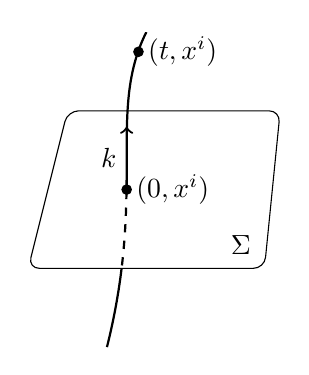
\begin{tikzpicture}
        \draw[rounded corners] (0,0) -- (0.5,2) -- (3.2,2) -- (3,0) -- cycle;
        \def\killingone{\draw[thick] (1,-1) .. controls (1.5,1) and (1,2) .. (1.5,3)}
        \begin{scope}
            \clip (0,0) rectangle (3,-1);
            \killingone;
        \end{scope}
        \begin{scope}[dashed]
            \clip (0,1) rectangle (3,0);
            \killingone;
        \end{scope}
        \begin{scope}
            \clip (0,1) rectangle (3,3);
            \killingone;
        \end{scope}
        \draw[fill] (1.25,1) circle (0.06) node[right] {\((0,x^i)\)};
        \draw[->,thick] (1.25,1) -- (1.25,1.8) node[midway,left] {\(k\)};
        \draw[fill] (1.4,2.75) circle (0.06) node[right] {\((t,x^i)\)};
        \node at (2.7,0.3) {\(\Sigma\)};
    \end{tikzpicture}
\end{wrapfigure}

Suppose we have a stationary spacetime with timelike Killing vector \(k\). Let \(\Sigma\) be a spacelike 3 dimensional hypersurface, and let \(x^i\), \(i=1,2,3\) be coordinates on \(\Sigma\).

We define coordinates for the manifold in the following way: from each point \((x^1,x^2,x^3)\) extend an integral curve of \(k\); the point \((t,x^i)\) is a parameter distance \(t\) along this curve.

In the chart \((t,x^i)\), we can write:
\begin{equation}
    k=\pdv{t}
\end{equation}
Then, using the defining property of Killing vectors, we have that the metric is independent of \(t\). Thus, we can write:
\begin{equation}
    \dd{s}^2 = g_{00}(x^k)\dd{t}^2 + 2g_{0i}(x^k)\dd{t}\dd{x^i} + g_{ij}(x^j)\dd{x^i}\dd{x^j}
\end{equation}
and we have \(g_{00}<0\) since \(k\) is timelike.

Suppose we have a surface \(\Sigma\) given by \(f(x)=0\), where \(f:\mathcal{M}\rightarrow\RR\), \(\dd{f}|_\Sigma\ne0\). Then \(\dd{f}\) is normal to \(\Sigma\). Suppose \(n\) is another 1-form that is normal to \(\Sigma\). Then we can write \(n=g\dd{f}+fn'\), where \(g\) is a function and \(n'\) is some 1-form. We have:
\begin{equation}
    \dd{n} = \dd{g}\wedge\dd{f}+g\underbrace{\dd[2]{f}}_{=0} + \dd{f}\wedge n' + f\dd{n'}
\end{equation}
\begin{equation}
    \implies \dd{n}|_\Sigma = (\dd{g}-n')\wedge\dd{f} \implies n\wedge \dd{n}|_\Sigma = 0
\end{equation}
In fact, the converse is true:
\begin{theorem}[Frobenius]
    If \(n\) is a 1-form such that \(n\wedge \dd{n}=0\), then there exist functions \(f,g\) such that \(n=g\dd{f}\), so that \(n\) is normal to surfaces of constant \(f\).
\end{theorem}
If \(n\) is a 1-form of this type, we say it is \emph{hypersurface-orthogonal}.

\begin{defn}
    \((\mathcal{M},g)\) is \emph{static} if it contains a hypersurface-orthogonal timelike KVF.
\end{defn}

Suppose we are in a static spacetime, and define coordinates \(t,x^i\) as before. \(\Sigma\) is a surface of constant \(t\), so we have \(k \propto dt\), \(k_\mu \propto (1,0,0,0)\). Also note that \(k_\mu = g_{\mu\nu}k^\nu = g_{\mu\nu}(\pdv{t})^\nu = (g_{00},g_{10},g_{20},g_{30})\). Hence we can deduce that \(g_{i0}=0\), and can write the metric as:
\begin{equation}
    \dd{s}^2 = g_{00}(x^k) \dd{t}^2 + g_{ij}(x^k)\dd{x^i}\dd{x^j}
\end{equation}
where as before \(g_{00}<0\). In this metric we have a discrete isometry \((t,x^i) \rightarrow (-t,x^i)\). A static metric must be time-independent \emph{and} invariant under time reversal. A simple case of a stationary but not static metric is that associated with a rotating star. If we reverse time the star spins in the other direction.

\subsection{Static, spherically symmetric spacetimes}
If we have a spacetime that is both stationary and spherically symmetric, then the isometry group must contain:
\begin{equation}
    \underbrace{\RR}_{\substack{\text{time}\\\text{translation}}} \times \underbrace{SO(3)}_{S^2 \text{ orbits}}
\end{equation}
It can be shown that with this condition the spacetime must also be static.

Let \(\Sigma_t \perp k^a\) be a foliation of the spacetime, and use coordinates \((r,\theta,\phi)\) on each surface, where \(\theta,\phi\) are the usual spherical coordinates and \(r\) is the area-radius function as defined earlier. Then we must have:
\begin{equation}
    \dd{s}^2|_{\Sigma_t} = e^{2\Psi(r)}\dd{r}^2 + r^2\dd{\Omega}
\end{equation}
for some function \(\Psi(r)\). Note that we have no \(\dd{r}\dd{\theta}\) or \(\dd{r}\dd{\phi}\) terms because they would violate spherical symmetry. If we define \(t\) as above we can then write the entire metric as:
\begin{equation}
    \dd{s}^2 = -e^{2\Phi(r)}\dd{t}^2 + e^{2\Psi(r)}\dd{r}^2 + r^2\dd{\Omega}
\end{equation}
for some other function \(\Phi(r)\).

\subsection{The TOV equations}
Consider now the matter inside a stationary and spherically symmetric star. We will model the star as a perfect fluid, which means we have the following energy-momentum tensor:
\begin{equation}
    T_{ab} = (\rho+P)u_au_b + \rho g_{ab}
\end{equation}
where \(\rho\) is the energy density, \(P\) is the pressure, and \(u_a\) is the 4-velocity of the fluid. Since the star is stationary, we can assume the fluid is at rest, so \(u^a = e^{-\Phi}\left( \pdv{t} \right)^a\) (since \(u\) is a unit vector pointing in the \(t\) direction). Also, since we have spherical symmetry we can assume that \(\rho\) and \(P\) are functions of \(r\) only.

\lecture{18/01/16}
Make the following definition:
\begin{equation}
    e^{2\Psi(r)} = \left( 1 - \frac{2m(r)}{r} \right)^{-1}
\end{equation}
Note that since \(e^{2\Psi(r)}>0\), we have \(m(r) < \frac{r}{2}\). Using the Einstein field equations \(G = 8\pi T\) it is now possible to derive the \emph{Tolman-Oppenheimer-Volkoff equations}:

\begin{equation}
    \dv{m}{r} = 4\pi r^2\rho
    \tag{TOV1}
    \label{TOV1}
\end{equation}
\begin{equation}
    \dv{\Phi}{r} = \frac{m+4\pi r^3P}{r(r-2m)}
    \tag{TOV2}
    \label{TOV2}
\end{equation}
\begin{equation}
    \dv{P}{r} = - (P+\rho) \frac{m+4\pi r^3P}{r(r-2m)}
    \tag{TOV3}
    \label{TOV3}
\end{equation}
We now have three equations, but four unknowns (\(m\),\(\Phi\),\(\rho\) and \(P\)). In order to solve this system, we will need a fourth equation, and the one most commonly chosen is an equation of state relating \(P\) and \(\rho\). In a cold star, we can assume that the temperature \(T(\rho,P)=0\) and we can solve this to get \(P\) explicitly in terms of \(\rho\):
\begin{equation}
    P = P(\rho)
\end{equation}
This is called a \emph{barotropic} equation of state.

We will assume that \(\rho,P>0\). We will also assume that \(\dv{P}{\rho}>0\); this is a stability condition\footnote{Consider \(\dv{P}{\rho}<0\). Then if \(\rho\) increases by a small amount in a region \(R\), \(P\) decreases in \(R\), but then this causes more fluid to flow into \(R\), increasing \(\rho\) further.}. 

Let the radius of the star be \(R\).
\begin{description}
    \item[Outside the star] (\(r>R\)) we can assume \(\rho = P = 0\). \eqref{TOV1} then gives that \(m(r) = M\) a constant. \eqref{TOV2} further provides that \(\Phi = \frac{1}{2}\log\left( 1-\frac{2M}{r} \right) + \Phi_0\), where \(\Phi_0\) is another constant. Note that since \(g_tt = -e^{2\Phi} \rightarrow e^{-2\Phi_0}\) as \(r\rightarrow\infty\), we can eliminate \(\Phi_0\) by making a change of coordinates \(t\rightarrow e^{\Phi_0}t\), so w.l.o.g. we assume that \(\Phi_0 = 0\).
        Hence we have the \emph{Schwarzschild metric}:
        \begin{equation}
            \dd{s}^2 = - \left( 1 - \frac{2M}{r} \right)\dd{t}^2 + \left( 1 - \frac{2M}{r} \right)^{-1}\dd{r}^2 + r^2\dd{\Omega}^2
        \end{equation}
        By taking \(r\) to be large and comparing with Newtonian gravity, we can deduce that \(M\) is in fact the mass of the star.
        Note that this metric has a problem. It is singular at the so-called \emph{Schwarzschild radius} \(r=2M\). Thus a static, spherically symmetric star must have \(R>2M\) (in a normal star, \(R\gg2M\)).
    \item[Inside the star] (\(r<R\)), we now have matter to deal with. Integrating \eqref{TOV1}, we have:
        \begin{equation}
            m(r) = 4\pi\int_0^r\rho(r')r'^2\dd{r'}+m_*
        \end{equation}
        where \(m_*\) is a constant. Consider a constant \(t\) hypersurface. The induced line element on this hypersurface is \(\dd{s}^2 = e^{2\Psi}\dd{r}^2 + r^2\dd{\Omega}^2\). The proper radius (i.e. distance to \(r=0\)) of a point is given by \(\int_0^re^{\Psi(r')}\dd{r'}\). In order for our spacetime to be a manifold, we require that it is locally flat at \(r = 0\), and this requires that the proper radius tends to the area-radius as \(r\rightarrow 0\). Note that
        \(\int_0^re^{\Psi(r')}\dd{r'} \sim e^{\Psi(0)}r\) as \(r\rightarrow 0\), so we require that \(e^{\Psi(0)} = 1\), or equivalently \(m(0) = 0\). From this we deduce that \(m_*=0\). 

        If we match this expression on the boundary of the star to the Schwarzschild solution for the exterior, we see that \(m(R)=M\), or:
        \begin{equation}
            M = 4\pi\int_0^R\rho(r)r^2\dd{r}
            \tag{\(*\)}
            \label{match}
        \end{equation}
        The volume form on a constant \(t\) hypersurface is \(e^\Psi r^2\sin\theta \dd{r}\wedge\dd{\theta}\wedge\dd{\phi}\), and so the energy of the matter in the star for \(t\) constant is:
        \begin{equation}
            E = 4\pi\int_0^R\rho e^\Psi r^2\dd{r}
        \end{equation}
        Note that since \(m\) is increasing, so is \(e^\Psi\) and hence \(e^\Psi\ge1\) for all \(0 \le r \le R\). Thus we have \(E > M\). The reason for this is that we have a gravitational binding energy \(E-M\).

        If we evaluate \(\frac{m(r)}{r}<\frac{1}{2}\) at \(r=R\) we see that \(\frac{M}{R} < \frac{1}{2}\). In fact it is possible to improve this: \eqref{TOV3} \(\implies\dv{P}{r}\le0\implies\dv{\rho}{r}\le0\), and from this we can deduce:
        \begin{equation}
            \frac{m(r)}{r} < \frac{2}{9}\left( 1 - 6\pi r^2P(r) + \left[ 1 + 6\pi r^2P(r) \right]^{\frac{1}{2}} \right)
            \tag{\(\dagger\)}
            \label{buchdahl}
        \end{equation}
        Setting \(r = R\) and noting \(P(R) = 0\), we obtain the so-called \emph{Buchdahl inequality}: \(\frac{M}{R}<\frac{4}{9}\).

        In general, we must solve this system of equations numerically. \eqref{TOV1} and \eqref{TOV3} are a pair of coupled first order ODEs for \(m(r)\) and \(\rho(r)\), from which we can obtain a unique solution given \(m(0)=0\) and specifying \(\rho(0) = \rho_c\), the central density. From \eqref{TOV3} we have that \(P\) is decreasing in \(r\), so \(R(\rho_c)\) is determined by fixing \(P(R) = 0\). Then, using \eqref{match} we can obtain \(M(\rho_c)\). Finally, using
        \eqref{TOV2} and the boundary condition that \(\Phi(R) = \frac{1}{2}\log\left( 1 - \frac{2M}{R} \right)\) we can deduce \(\Phi(r)\). 

        To summarise, given an equation of state, static, spherically symmetric, cold stars are a 1-parameter family labelled by \(\rho_c\).
\end{description}

\subsection{Maximum mass}
We wish to find a limit on the maximum mass of a star.
\begin{figure}[H]
    \centering
    \begin{tikzpicture}[scale=1.5]
        \draw[domain=0:3,smooth,variable=\x] plot({\x},{\x*(3.2-\x)/2});
        \draw[thick,->] (0,0) -- (3.5,0) node[right] {\(\rho_c\)};
        \draw[thick,->] (0,0) -- (0,1.6) node[above] {\(M\)};
        \draw[dashed] (0,1.28) node[left] {\(M_{\text{max}}\)} -- (3.5,1.28);
    \end{tikzpicture}
\end{figure}
In general, \(M_{\text{max}}\) depends on the equation of state, but here we run into a problem: we do not know the equation of state in certain conditions, namely \(\rho>\rho_0\), where \(\rho_0\) is typically on the order of the density of an atomic nucleus.

\begin{wrapfigure}{l}{0.5\linewidth}
    \centering
    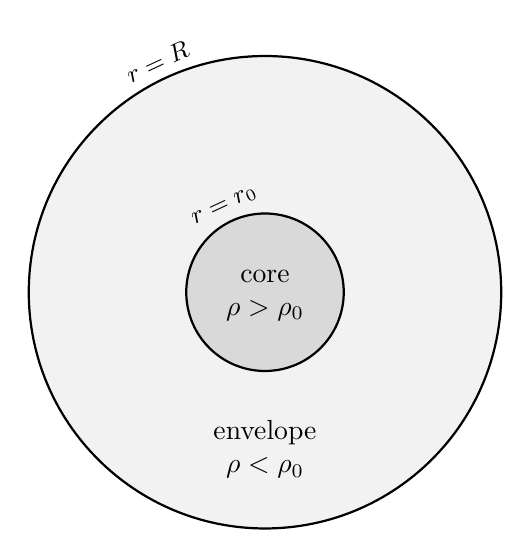
\begin{tikzpicture}
        \fill[gray!10] (0,0) circle (3);
        \fill[gray!30] (0,0) circle (1);
        \draw[thick] (0,0) circle (3);
        \draw[thick] (0,0) circle (1);

        \node at (0,0) {
            \begin{tabular}{c}
                core \\
                \(\rho>\rho_0\)
            \end{tabular}
            };
        \node at (0,-2) {
            \begin{tabular}{c}
                envelope \\
                \(\rho<\rho_0\)
            \end{tabular}
            };
        
        \node[above,rotate=25,shift={(0,1)}] at (0,0) {\small\(r=r_0\)};
        \node[above,rotate=25,shift={(0,3)}] at (0,0) {\small\(r=R\)};
    \end{tikzpicture}
\end{wrapfigure}
Remarkarbly, it is still possible to find an upper bound on the mass of a star. We do this by splitting the star into two regions: an \emph{envelope}, in which we know the equation of state (so \(\rho<\rho_0\)), and a \emph{core}, in which we do not (\(\rho>\rho_0\)). Since \(\dv{\rho}{r}<0\), the envelope does in fact envelope the core.

Let \(m_0 = m(r_0)\); we call this the \emph{core mass}. Since the minimum density in the core is \(\rho_0\), we have \(m_0\ge\frac{4}{3}\pi r_0^3\rho_0\). Additionally, we can apply \eqref{buchdahl} at \(r=r_0\) to obtain:
\begin{equation}
    \frac{m_0}{r_0} < \frac{2}{9}\left( 1 - 6\pi r_0^2P_0 + \left[ 1 + 6\pi r_0^2P_0 \right]^{\frac{1}{2}} \right)
\end{equation}
where \(P_0=P(\rho_0)\). This is a decreasing function of \(P_0\), so \(\frac{m_0}{r_0}<\frac{4}{9}\).

Lets plot these two constraints:
\begin{figure}[H]
    \centering
    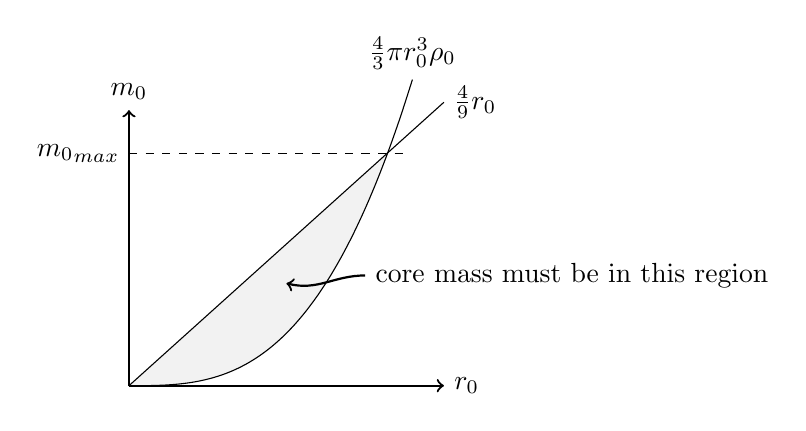
\begin{tikzpicture}
        \begin{scope}
            \clip (0,0) -- (4,0) -- (4,3.6) -- cycle;
            \fill[gray!10,domain=0:3.6,smooth,variable=\x] plot({\x},{\x^3/12});
        \end{scope}
        \draw[domain=0:3.6,smooth,variable=\x] plot({\x},{\x^3/12}) node[above] {\(\frac{4}{3}\pi r_0^3\rho_0\)};
        \draw[domain=0:4,smooth,variable=\x] plot({\x},{\x*0.9}) node[right] {\(\frac{4}{9}r_0\)};
        \draw[thick,->] (0,0) -- (4,0) node[right] {\(r_0\)};
        \draw[thick,->] (0,0) -- (0,3.5) node[above] {\(m_0\)};
        \draw[dashed] (0,2.95) node[left] {\({m_0}_{\text{max}}\)} -- (3.5,2.95);

        \draw[thick,<-] (2,1.3) .. controls (2.4,1.2) and (2.6,1.4) .. (3,1.4) node[right] {core mass must be in this region};
    \end{tikzpicture}
\end{figure}
We see that we have an upper bound on the core mass. Solving for this upper bound, we find:
\begin{equation}
    m_0 < \sqrt{\frac{16}{23\pi\rho_0}}
\end{equation}
If \(\rho_0\approx\) nuclear density, then we have \(m_0 \lesssim 5M_{\astrosun}\).

Now we can extend our solution to the envelope. \(m_0\) and \(r_0\) together uniquely determine the envelope, as we can solve \eqref{TOV1} and \eqref{TOV3} starting at \(r=r_0\) and using the known equation of state for \(\rho<\rho_0\). From this we obtain \(M\) as a function of \(m_0\) and \(r_0\), and so can find the maximal value of \(M\) when \(m_0,r_0\) take values in the region in the graph above.

Numerically, we can find that \(M\) is maximised when \(m_0\) is maximised, and that the maximum mass is \(M\approx m_0\approx5M_{\astrosun}\).

In fact, it is possible to improve this limit by imposing that the speed of sound is physical, i.e.\ less than the speed of light: \(\sqrt{\dv{P}{\rho}}\le1\). Using this gives \(M \lesssim 3M_{\astrosun}\).

\section{The Schwarzschild solution}
\lecture{20/01/16}
We showed earlier that the only static, spherically symmetric solution of the vacuum EFEs is the Schwarzschild solution:
\begin{equation}
    \dd{s}^2 = - \left( 1-\frac{2M}{r} \right)\dd{t}^2 + \left( 1-\frac{2M}{r} \right)^{-1}\dd{r}^2 + r^2\dd{\Omega}^2
\end{equation}
\(t,r,\theta,\phi\) are known as \emph{Schwarzschild coordinates}. We will assume \(M>0\).

In fact:
\begin{theorem}[Birkhoff]
    Any spherically symmetric solution of the vacuum Einstein equations is isometric to the Schwarzschild solution.
\end{theorem}
So in particular, spherical symmetry and a vacuum implies a static spacetime (for \(r>2M\)).

\subsection{Gravitational redshift}
Consider two fixed observers \(A,B\) in a Schwarzschild spacetime. \(A\) sends two photons to \(B\), seperated by a time \(\Delta t\).

\begin{wrapfigure}{l}{0.4\linewidth}
    \centering
    \begin{tikzpicture}
        \draw[thick,->] (-1.5,-1.5) -- (-0.8,-1.5) node[right] {\(r\)};
        \draw[thick,->] (-1.5,-1.5) -- (-1.5,-0.8) node[above] {\(t\)};
        \draw[thick] (0,0) -- (0,-4) node[below] {\(A\)};
        \draw[thick] (3,0) -- (3,-4) node[below] {\(B\)};
        \fill (0,-3) circle (0.07);
        \fill (3,-1.5) circle (0.07);
        \fill (0,-2.5) circle (0.07);
        \fill (3,-1) circle (0.07);
        \draw[photon] (0,-3) -- (3,-1.5);
        \draw[photon] (0,-2.5) -- (3,-1);
        \draw[thick,<->] (-0.2,-3) -- (-0.2,-2.5) node[midway,left] {\(\Delta t\)};
        \draw[thick,<->] (3.2,-1.5) -- (3.2,-1) node[midway,right] {\(\Delta t\)};
    \end{tikzpicture}
\end{wrapfigure}
Because \(\pdv{t}\) is an isometry of the spacetime, the second photon's path is the same as that of the first, but translated by \(\Delta t\). Consider the 4-velocity of a fixed observer. We have:
\begin{equation}
    -1 = u^\mu u_\mu = g_{tt}\left(\dv{t}{\tau}\right)^2 = - \left( 1-\frac{2M}{r} \right)\left(\dv{t}{\tau}\right)^2
\end{equation}
Hence we have \(\dd{\tau} = \sqrt{1 - \frac{2M}{r}}\dd{t}\). Therefore the proper time intervals between the photons at \(A\) and \(B\) are:
\begin{equation}
    \Delta\tau_A = \sqrt{1-\frac{2M}{r_A}}\Delta t
    ,\quad
    \Delta\tau_B = \sqrt{1-\frac{2M}{r_B}}\Delta t
\end{equation}
So we have:
\begin{equation}
    \frac{\Delta \tau_B}{\Delta \tau_A} = \frac{\sqrt{1 - \frac{2M}{r_B}}}{\sqrt{1-\frac{2M}{r_A}}}
\end{equation}
If we suppose that the photons were sent at two subsequent wavecrests, then \(\Delta \tau\) is the period of the waves, equal to \(\lambda\), the wavelength (since \(c=1\)). We define the redshift \(z\) by:
\begin{equation}
    1 + z = \frac{\lambda_B}{\lambda_A} = \frac{\sqrt{1 - \frac{2M}{r_B}}}{\sqrt{1-\frac{2M}{r_A}}}
\end{equation}
For \(r_B > r_A\), we have \(z>0\), so light is redshifted as it climbs out of the gravitational field. For \(r_B\gg 2M\):
\begin{equation}
    1 + z = \sqrt{\frac{1}{1 - \frac{2M}{r_A}}}
\end{equation}
Note that this \(\rightarrow \infty\) as \(r_A\rightarrow2M\).

For a star, we have the Buchdahl inequality, \(R>\frac{9}{4}M\), so plugging this into the above, we find that the maximum redshift from the surface of a spherical star is \(z=2\).

\subsection{Geodesics}
Suppose \(x^\mu(\tau)\) is an affinely parametrised geodesic, and let its 4-velocity be \(u^\mu = \dv{x^\mu}{\tau}\). We have Killing fields \(k=\pdv{t}\) and \(m=\pdv{\phi}\), so along geodesics we have two conserved quantities:
\begin{equation}
    E=-k\vdot u = \left( 1-\frac{2M}{r} \right)\dv{t}{\tau}
    \qq{and}
    h = m\vdot u = r^2\sin^2\theta\dv{\phi}{\tau}
\end{equation}
If our geodesic is timelike and we choose \(\tau\) to be proper time, we can identify \(E\) as the energy per unit mass and \(h\) as the angular momentum per unit mass associated with the geodesic.

In the null case, we can define the \emph{impact parameter} \(b = \left|\frac{h}{E}\right|\), and identify this as the limit of the distance between the geodesic and the star perpendicular to the geodesic as \(r\rightarrow 0\).
\begin{figure}[H]
    \centering
    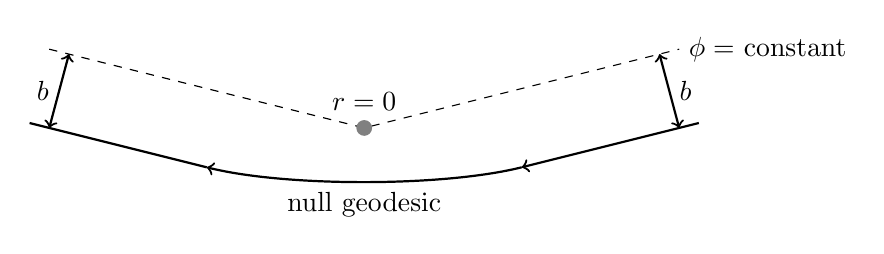
\begin{tikzpicture}
        \draw[dashed] (-4,1) -- (0,0) -- (4,1) node[right] {\(\phi = \) constant};
        \fill[gray] (0,0) circle (0.1);
        \node[above] at (0,0.1) {\(r=0\)};
        \draw[thick,->] (4.25,0.0625) -- (2,-0.5); 
        \draw[thick,->] (2,-0.5) .. controls (1,-0.75) and (-1,-0.75) .. (-2,-0.5) node[below, midway] {null geodesic};
        \draw[thick] (-2,-0.5) -- (-4.25,0.0625);
        \draw[thick,<->] (3.75,0.9375) -- (4,0) node[midway,right] {\(b\)};
        \draw[thick,<->] (-3.75,0.9375) -- (-4,0) node[midway,left] {\(b\)};
    \end{tikzpicture}
\end{figure}

equationéeieieieieiee

Exercises:
\begin{enumerate}
    \item Derive the Euler-Lagrange equation for \(\theta(\tau)\). Show that one can choose coordinates such that \(\theta(\tau) = \frac{\pi}{2}\), so that motion is contained in the equatorial plane.
    \item Rearrange the definition of proper time:
        \begin{equation}
            g_{\mu\nu}u^\mu u^\nu = \sigma = 
            \begin{cases}
                1 & \text{timelike}\\
                0 & \text{null}\\
                -1 & \text{spacelike}
            \end{cases}
        \end{equation}
        to obtain \(\frac{1}{2}\left( \dv{r}{\tau} \right)^2 + V(r) = \frac{1}{2}E^2\), where \(V(r) = \frac{1}{2}\left( 1-\frac{2M}{r} \right)\left( \sigma+\frac{h^2}{r^2} \right)\).
\end{enumerate}

\subsection{Eddington-Finkelstein coordinates}
Consider radial null geodesics (\(\sigma=0\)) in \(r>2M\). Since \(\phi\) is constant, we have \(h=0\) and so \(V=0\). Since we are dealing with a null geodesic, we are free to scale \(\tau\) such that \(E=1\). Hence we have:
\begin{equation}
    \dv{t}{\tau} = \left( 1-\frac{2M}{r} \right)^{-1}
    ,\quad
    \dv{r}{\tau} = \pm 1
\end{equation}
where the sign in the second equation depends on whether the geodesic is outgoing or ingoing. One thing of note is that an ingoing geodesic reaches \(r=2M\) in finite \(\tau\). The same is not true of \(t\):
\begin{equation}
    \dv{t}{r} = \pm\left( 1-\frac{2M}{r} \right)^{-1}
\end{equation}
so \(t\rightarrow\mp\infty\) as \(r\rightarrow2M\).

Define \(r_*=r+2M\log\abs{\frac{r}{2M}-1}\), \(\dd{r_*} = \frac{\dd{r}}{1 - \frac{2M}{r}}\) (\(*\)).

\begin{wrapfigure}{l}{0.3\linewidth}
    \centering
    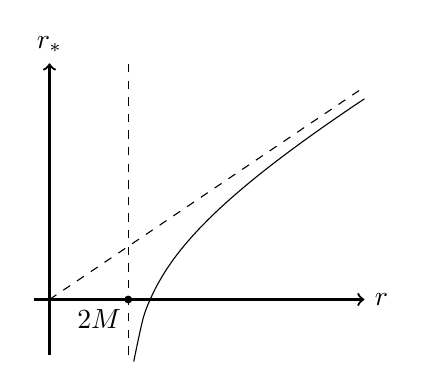
\begin{tikzpicture}
        \draw[thick,->] (0,-.7) -- (0,3) node[above] {\(r_*\)};
        \draw[thick,->] (-.2,0) -- (4,0) node[right] {\(r\)};
        \draw[domain=1.07:4,smooth,variable=\x] plot({\x},{(\x+ln(\x-1))/2});
        \draw[dashed] (0,0) -- (4,2.7);
        \draw[dashed] (1,-.7) -- (1,3);
        \fill (1,0) circle (0.05);
        \node[below] at (0.63,0) {\(2M\)};
    \end{tikzpicture}
\end{wrapfigure}
We have \(\dv{t}{r_*} = \pm1\), so \(t\mp r_*\) is a constant. Define \mbox{\(v = t + r_*\) (\(\dagger\))}, a constant along ingoing radial geodesics. The ingoing \emph{Eddington-Finklestein} coordinates are \(v,r,\theta,\phi\). In these coordinates, the line element is given by:
\begin{equation}
    \dd{s}^2 = - \left( 1-\frac{2M}{r} \right)\dd{v}^2 + 2\dd{v}\dd{r} + r^2\dd{\Omega}^2
\end{equation}
This is smooth for all \(r > 0\). In matrix form, the metric is:
\begin{equation}
    g_{\mu\nu} = 
    \begin{pmatrix}
        - \left( 1 - \frac{2M}{r} \right) & 1 & 0 & 0 \\
        1 & 0 & 0 & 0 \\
        0 & 0 & r^2 & 0 \\
        0 & 0 & 0 & r^2\sin^2\theta
    \end{pmatrix}
\end{equation}
We have \(g = \det g_{\mu\nu} = -r^4\sin^2\theta\), so \(g_{\mu\nu}\) is non-degenerate for all \(r > 0\) and furthermore it is Lorentzian for all \(r>0\).

In summary, spacetime can be extended through \(r=2M\) to a new region \(r<2M\).

Exercise: for \(0<r<2M\), define \(r_*\) by (\(*\)) and \(t\) by (\(\dagger\)). Show that the metrix in coordinates \(t,r,\theta,\phi\) is the Schwarzschild metric with \(0<r<2M\).

So for a ingoing radial null geodesic inside \(r=2M\) we have \(\dv{r}{\tau}=-1\), so it reaches \(r=0\) in finite \(\tau\).

Consider \(R_{abcd}R^{abcd}\). Some work will lead to:
\begin{equation}
    R_{abcd}R^{abcd} \propto \frac{M^2}{r^6} \rightarrow \infty \text{ as } r\rightarrow0
\end{equation}
This quantity is a scalar, so it diverges in any coordinate system. We call \(r=0\) a \emph{curvature singularity}. There are infinite tidal forces at \(r=0\). Note that \(r=0\) is not a part of the our spacetime, because \(g_{ab}\) is not defined there.

For \(r>2M\) we have the ``static'' KVF \(\pdv{t}\). In Eddington-Finklestein coordinates \(x^\mu\), we have:
\begin{equation}
    k = \pdv{x^\mu}{t}\pdv{x^\mu} = \pdv{v}
\end{equation}
Also, \(k^2 = g_{vv} = -\left( 1-\frac{2M}{r} \right)\), so \(k\) is null at \(r=2M\), and spacelike at \(r < 2M\). Only \(r > 2M\) is static.

\subsection{Finklestein diagram}
\lecture{22/01/16}
Consider outgoing radial null geodesics in \(r>2M\). We have \(t-r_*= \text{constant}\), so:
\begin{equation}
    v = 2r_* + \text{constant}
    = 2r + 4M\log\left|\frac{r}{2M}-1\right| + \text{constant}
    \tag{\(*\)}
    \label{sociable}
\end{equation}
Exercise: Consider null geodesics in ingoing Eddington-Finklestein coordinates and show that these fall into 2 families: ingoing with \(v = \text{constant}\), and outgoing either of the form \eqref{sociable} or \(r=2M\). 

Let \(t^*=v-r\). We can draw the radial null geodesics in a \emph{Finklestein diagram}:
\begin{figure}[H]
    \centering
    \begin{tikzpicture}
        \begin{scope}[thick, decoration={
            markings,
            mark=at position 0.5 with {\arrow{latex}}}
            ] 
            \clip (0,-3) rectangle (6,4);
            \begin{scope}[red]
                \draw[domain=3.07:6,smooth,variable=\x,postaction=decorate] plot({\x},{3*(ln(\x/3 - 1)+2)});
                \draw[domain=3.3:6,smooth,variable=\x,postaction=decorate] plot({\x},{3*(ln(\x/3 - 1)+1)});
                \draw[domain=3.6:6,smooth,variable=\x,postaction=decorate] plot({\x},{3*(ln(\x/3 - 1)+0.2)});

                \draw[domain=3.07:6,smooth,variable=\x,postaction=decorate] plot({6 - \x},{3*(ln(\x/3 - 1)+2)});
                \draw[domain=3.3:6,smooth,variable=\x,postaction=decorate] plot({6-\x},{3*(ln(\x/3 - 1)+1)});
                \draw[domain=3.6:6,smooth,variable=\x,postaction=decorate] plot({6-\x},{3*(ln(\x/3 - 1)+0.2)});
            \end{scope}
            \begin{scope}[blue]
                \draw[shift={(1,1)},postaction=decorate] (5.5,-10) -- (-6.5,4);
                \draw[shift={(2,2)},postaction=decorate] (5.5,-10) -- (-6.5,4);
                \draw[shift={(3,3)},postaction=decorate] (5.5,-10) -- (-6.5,4);
                \draw[shift={(4,4)},postaction=decorate] (5.5,-10) -- (-6.5,4);
                \draw[shift={(5,5)},postaction=decorate] (5.5,-10) -- (-6.5,4);
                \draw[shift={(6,6)},postaction=decorate] (5.5,-10) -- (-6.5,4);
            \end{scope}
        \end{scope}

        \draw[thick,->] (0,0) -- (6,0) node[right] {\(r\)};
        \draw[thick,->] (0,-3) -- (0,4) node[midway,above,sloped] {curvature singularity};
        \node[above] at (0,4) {\(t^*\)};
        \node[right,fill=white] at (3,-0.3) {\(2M\)};
        \draw[dashed, thick] (3,-3) -- (3,4);

        \node[right,rotate=-45, blue] at (6,2.5) {ingoing};
        \node[right,rotate=45, red] at (6,3) {outgoing};

        \newcommand{\lightcone}[4]{\
            \begin{scope}[shift={(#1,#2)}, scale=0.3, rotate=#4, semithick]
                \draw ({-sin(#3)},{-cos(#3)}) -- ({sin(#3)},{cos(#3)});
                \draw ({sin(#3)},{-cos(#3)}) -- ({-sin(#3)},{cos(#3)});
                \draw (0,{-cos(#3)}) ellipse ({sin(#3)} and {0.3*sin(#3)});
                \draw (0,{cos(#3)}) ellipse ({sin(#3)} and {0.3*sin(#3)});
            \end{scope}
        }

        \lightcone{2.6}{-0.1}{20}{23.5}
        \lightcone{1.98}{2.77}{10}{30}
        \lightcone{3.57}{0.93}{27}{15}
    \end{tikzpicture}
\end{figure}
In \(r < 2M\), \(r\) decreases along both families, and we reach \(r=0\) in finite \(\tau\). In fact we will show later that \(r\) decreases along \emph{any} timelike or null curve in \(r<2M\). Equipped with this knowledge we can make a rough definition of a \emph{black hole} as a region of space from which no signal can reach ``infinity''.

\subsection{Gravitational collapse}
The surface of a collapsing star follows a timelike geodesic, and we can plot this on a Finklestein diagram:
\begin{figure}[H]
    \centering
    \begin{tikzpicture}
        \begin{scope}[thick, shift={(-1,0)}, decoration={
            markings,
            mark=at position 0.5 with {\arrow{latex}}}
            ] 
            \clip (0,-3) rectangle (6,4);
            \begin{scope}[red]
                \draw[domain=3.07:9,smooth,variable=\x,postaction=decorate] plot({\x},{3*(ln(\x/3 - 1)+2)});
                \draw[domain=3.3:9,smooth,variable=\x,postaction=decorate] plot({\x},{3*(ln(\x/3 - 1)+1)});
                \draw[domain=3.6:9,smooth,variable=\x,postaction=decorate] plot({\x},{3*(ln(\x/3 - 1)+0.2)});

            \end{scope}
        \end{scope}

        \fill[gray!20] (0,-3) -- (0,3.5)
            .. controls (4,2.5) and (3.5,-2) .. (4,-3) -- cycle;

        \draw[thick,->] (0,0) -- (5,0) node[right] {\(r\)};
        \draw[thick,->] (0,-3) -- (0,4) node[midway,above,sloped] {curvature singularity};
        \node[above] at (0,4) {\(t^*\)};
        \node[right] at (2,-0.3) {\(2M\)};
        \draw[dashed, thick] (2,-3) -- (2,4);
        \draw (0,3.5) .. controls (4,2.5) and (3.5,-2) .. (4,-3);

        \draw[thick,<-] (3.3,-1.7) -- (4.2,-1.7) node[right]{stellar interior (not Schwarzschild)};
    \end{tikzpicture}
\end{figure}

It will be shown in the first example sheet that the total proper time along a timelike curve with \(r \le 2M\) can't exceed \(\pi M\), so a star collapses from \(r=2M\) to \(r=0\) within a proper time \(\pi M\) (this is about \SI{e-5}{\second} for \(M=M_{\astrosun}\). When this happens, a distant observer never sees the star cross \(r=2M\) -- it just redshifts away.

\subsection{Black hole region}
\begin{defn}
    A non-zero vector is \emph{causal} if it is timelike or null. A curve is \emph{causal} if its tangent vector is everywhere causal. 
\end{defn}
\begin{defn}
    A spacetime is \emph{time-orientable} if is admits a \emph{time orientation}, i.e.\ a causal vector field \(T^a\).
\end{defn}
\begin{defn}
    A \emph{future-directed} causal vector is one that lies in the same lightcone as the time orientation \(T^a\); a \emph{past-directed} causal vector is one that does not.
\end{defn}
Given a time orientation \(T^a\), we always have a second inequivalent time orientation \(-T^a\).

For \(r>2M\) Schwarzschild, the obvious choice of time orientation is \(k=\pdv{t}\). However, \(k=\pdv{v}\) is not causal for \(r<2M\). In ingoing Eddington-Finklestein coordinates, \(\pm\pdv{r}\) is null, since \(g_{rr} = 0\). We can choose either of these as a time orientation, but we want to pick a sign that agrees with \(k\) for \(r>2M\). We have:
\begin{equation}
    k\vdot\left( \pm \pdv{r} \right) = \pm g_{vr} = \pm 1
\end{equation}
Thus we use \(-\pdv{r}\) as the time orientation.

\begin{lemma}
    Let \(x^\mu(\lambda)\) be a future-directed causal curve. If \(r(\lambda_0) \le 2M\), then \(r(\lambda) \le 2M\) for all \(\lambda \ge \lambda_0\).
\end{lemma}
\begin{proof}
    Let \(V^\mu = \dv{x^\mu}{\lambda}\). \(V^\mu\) is future-directed. Thus we have:
    \begin{align}
        0 \le \left( -\pdv{r} \right)\vdot V = -g_{r\mu}V^\mu = -V^v = - \dv{v}{\lambda}
    \end{align}
    and so:
    \begin{align}
        & V^2 = -\left(1-\frac{2M}{r}\right) \left( \dv{v}{\lambda} \right)^2 + 2 \dv{v}{\lambda}\dv{r}{\lambda} + r^2 \left( \dv{\Omega}{\lambda} \right)^2 \\
        \implies & -2\dv{v}{\lambda}\dv{r}{\lambda} = \underbrace{-V^2}_{\ge0} - \left( 1-\frac{2M}{r} \right)\left( \dv{v}{\lambda} \right)^2 + \underbrace{r^2\left( \dv{\Omega}{\lambda} \right)^2}_{\ge0}
    \end{align}
    Thus if \(r \le 2M\), we have \(\dv{v}{\lambda}\dv{r}{\lambda}\le0\). 
    
    Suppose \(r \le 2M\) and \(\dv{r}{\lambda} > 0\). Then since \(\dv{v}{\lambda}\le 0\) we must have \(\dv{v}{\lambda} = 0\), and hence \(V^2 = 0 = \dv{\Omega}{\lambda}\). The only non-zero component of \(V\) is \(V^r = \dv{r}{\lambda}>0\), so \(V\) is a positive multiple of \(\pdv{r}\), but this implies that \(V\) is past-directed, which is a contradiction.

    Hence we have \(\dv{r}{\lambda} \le 0\) if \(r \le 2M\), and we can show similarly \(\dv{r}{\lambda} < 0\) if \(r < 2M\). Hence if \(r(\lambda_0) < 2M\), then \(r(\lambda)\) is monotonically decreasing for \(\lambda \ge \lambda_0\). \disapprove
\end{proof} 

\subsection{Detecting black holes}
Black holes have two recognizable qualities:
\begin{itemize}
    \item Unlike in the case of cold stars, there is no upper bound on the mass of a black hole.
    \item Black holes are very small for a given mass.
\end{itemize}

One interesting case is that of the \emph{supermassive black holes}. No one knows how they form...

\subsection{Orbits around black holes}
\lecture{25/01/16}
Comsider timelike geodesics, and recall the orbital equation of a Schwarzschild black hole:
\begin{equation}
    \frac{1}{2}\left( \dv{r}{\tau} \right)^2 + V(r) = \frac{1}{2}E^2
    \qq{where}
    V(r) = \frac{1}{2}\left( 1-\frac{2M}{r} \right)\left( 1 + \frac{h^2}{r^2} \right)
\end{equation}
It can easily be shown that \(V'(r)=0\) if \(r = r_\pm = \frac{h^2\pm\sqrt{h^4-12h^2M^2}}{2M}\). Lets plot \(V\):

\begin{figure}[H]
    \centering
    \begin{tikzpicture}
        \draw[->, thick] (0,0) -- (6,0) node[right] {\(r\)};
        \draw[->, thick] (0,-1) -- (0,4) node[above] {\(V\)};
        \draw (0.5,-1) .. controls (0.7,0) and (1,3.5) .. (2,3.5)
            .. controls (2.5,3.5) and (3,2.5) .. (3.5,2.5)
            .. controls (4,2.5) and (4,2.9) .. (6,2.95);
        \draw[dashed] (0,3) node[left] {\(\frac{1}{2}\)} -- (6,3);
        \draw[dashed] (2,0) node[below] {\(r_-\)} -- (2,3.5);
        \draw[dashed] (3.5,0) node[below] {\(r_+\)} -- (3.5,2.5);

        \node[right] at (7.5,2.25) {\(r=r_+\) is a stable circular orbit};
        \node[right] at (7.5,1.75) {\(r=r_-\) is an unstable circular orbit};
    \end{tikzpicture}
\end{figure}
It is a simple exercise to show that \(3M < r_- < 6M < r_+\). We call \(r=6M\) the \emph{innermost stable circular orbit} (ISCO).

Suppose \(r=r_\pm\), then we have a circular orbit \(\dv{r}{\tau} = 0\), and we can show:
\begin{equation}
    \frac{E^2}{2}=V(r) \implies E = \frac{r-2M}{r^{\frac{1}{2}}(r-3M)^{\frac{1}{2}}} \approx 1 - \frac{M}{2r} \text{ for } r\gg2M
\end{equation}
Hence we have that the energy of a distant orbit is approximately \(m-\frac{Mm}{2r}\). \(m\) is the rest mass energy of the orbiting particle, and \(\frac{Mm}{2r}\) is the gravitational binding energy of its orbit.

\begin{wrapfigure}{r}{0.4\linewidth}
    \centering
    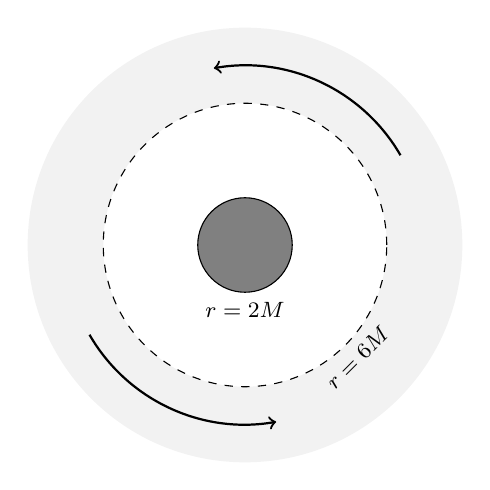
\begin{tikzpicture}[scale=1.2]
        \fill[gray!10] (0,0) circle (2.3);
        \fill[white] (0,0) circle (1.5);
        \fill[gray] (0,0) circle (0.5);
        \draw (0,0) circle (0.5);
        \draw[dashed] (0,0) circle (1.5);

        \draw[thick,->] ({1.9*cos(30)},{1.9*sin(30)}) arc (30:100:1.9);
        \draw[thick,->] ({1.9*cos(-150)},{1.9*sin(-150)}) arc (-150:-80:1.9);

        \node[below,rotate=45] at ({1.5*cos(45)},{-1.5*sin(45)}) {\footnotesize\(r=6M\)};
        \node[below] at (0,-0.5) {\footnotesize\(r=2M\)};
    \end{tikzpicture}
\end{wrapfigure}
When a star orbits around a black hole, the black hole robs the star of matter, forming an \emph{accretion disc} around the black hole. As a first approximation we will assume that particles in this accretion disc follow stable circular orbits of the form above. Friction between the particles causes their \(E\) to decrease, and hence their \(r\) to also decrease, and so these particles will fall towards the ISCO, where they will then fall into the black hole.

At \(r\to\infty\) we have \(E = 1\), and at the ISCO we have \(E=\sqrt{\frac{8}{9}}\). Thus the proportion of lost to friction (and then radiated away as x-rays) is \(1-\sqrt{\frac{8}{9}}\approx6\%\).

\subsection{White holes}
Consider again the region \(r>2M\), and let \(u = t-r_*\). We define the \emph{outgoing} Eddington-Finklestein coordinates as \(u,r,\theta,\phi\). In these coordinates, the line element is given by:
\begin{equation}
    \dd{s}^2=-\left( 1 - \frac{2M}{r} \right)\dd{u}^2-2\dd{u}\dd{r} + r^2\dd{\Omega}^2
\end{equation}
Since \(g_{\mu\nu}\) is smooth and \(\det g \ne 0\) for all \(r>0\), we can extend this to \(0 < r \le 2M\), and again we have a curvature singularity at \(r=0\). However it is important to note that this is not the same \(r < 2M\) region as before! To see this, consider outgoing radial null geodesics which have \(u\) constant and \(\dv{r}{\tau} = +1\). These have \(r\) increasing through \(r=2M\), in direct contradiction with the previous case. \(r < 2M\) is \emph{not} a black hole.

Exercise: show (i) \(k=\pdv{u}\), (ii) the time orientation equivalent to \(k\) for \(r\gg2M\) is \(+\pdv{r}\).

\(r<2M\) is known as a \emph{white hole region}; it is a region into which no signal from infinity can enter. In a certain sense a white hole is the time reversal of a black hole: \(u\mapsto -v\) is an isometry mapping outgoing Eddington-Finklestein coordinates to ingoing Eddington-Finklestein coordinates, but it does not preserve the time-orientation.

\subsection{Kruskal extension}
Consider \(r>2M\) Schwarzschild spacetime. We define \emph{Kruskal-Szekeres} coordinates \((U,V,\theta,\phi)\) by
\begin{equation}
    U = -e^{-u/4M} < 0
    \qq{and}
    V = e^{v/4M} > 0.
\end{equation}
We have
\begin{equation}
    UV = -e^{r_*/2M} = - e^{r/2M}\left( \frac{r}{2M} - 1 \right),
    \tag{\(**\)}
    \label{uv}
\end{equation}
which is monotonic and thus determines \(r = r(U,V)\). Similarly, 
\begin{equation}
    \frac{V}{U} = -e^{t/2M}
\end{equation}
determines \(t = t(U,V)\).

Exercise: show that the metric in Kruska-Szekeres coordinates is given by
\begin{equation}
    \dd{s}^2 = -\frac{32M^3e^{-r(U,V)/2M}}{r(U,V)} \dd{U}\dd{V} + r(U,V)^2 \dd{\Omega}^2.
\end{equation}
We use \eqref{uv} to define \(r(U,V)\) for \(U\ge0\) or \(V\le0\). We can analytically extend the spacetime with \(\det g \ne0\) through \(U=0\) or \(V=0\) to new regions with \(U\ge0\) or \(V\le0\). \(r=2M\) corresponds to two surfaces \(U=0\) and \(V=0\), intersecting at \(U=V=0\). \(r=0\) corresponds to a hyperbola with 2 branches. Ingoing and outgoing geodesics are described by \(V\), \(U\) constant respectively. We can plot thse features on a \emph{Kruskal diagram}:

\begin{figure}[H]
    \centering
    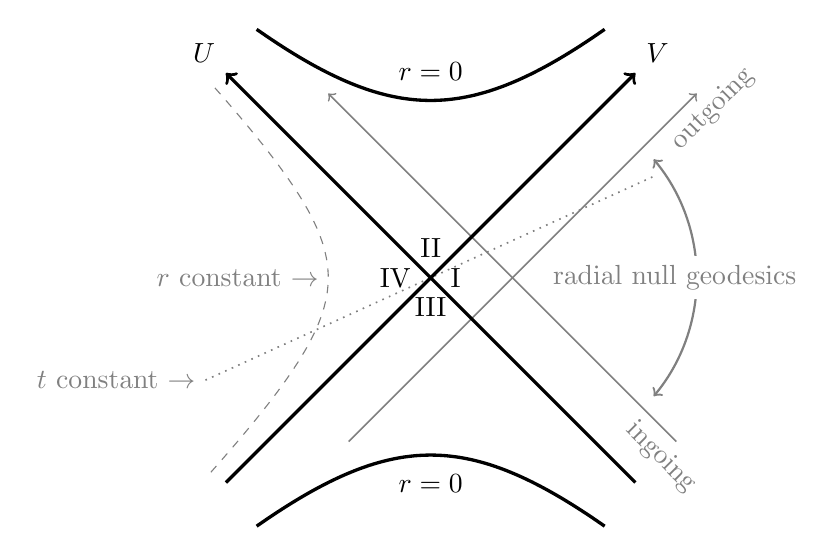
\begin{tikzpicture}[scale=1.3]
        \begin{scope}[gray]
            \draw[domain=-1.9:1.9,smooth,variable=\x,dashed] plot({-sqrt(1+\x*\x))},{\x});
            \node[left] at (-1,0) {\(r\) constant \(\rightarrow\)};

            \draw[dotted, semithick] (-2.2,-1) -- (2.2,1) node[left, at start] {\(t\) constant \(\rightarrow\)};

            \draw[semithick, <-] (-1,1.8) -- (2.4,-1.6) node[below, at end, sloped] {ingoing};
            \draw[semithick, <-] (2.6,1.8) -- (-0.8,-1.6) node[below, at start, sloped] {outgoing};
            \draw[thick, ->] (2.6,0) arc (0:40:1.8);
            \draw[thick, ->] (2.6,0) arc (0:-40:1.8);
            \node[right, fill=white] at (1.1,0) {radial null geodesics};
        \end{scope}

        \draw (0.1,0) node[right] {I};
        \draw (0,0.1) node[above] {II};
        \draw (0,-0.1) node[below] {III};
        \draw (-0.1,0) node[left] {IV};

        \draw[domain=-1.7:1.7,smooth,variable=\x,very thick] plot({\x},{sqrt(3+\x*\x))});
        \node[above] at (0,{sqrt(3)+0.1}) {\(r=0\)};
        \draw[domain=-1.7:1.7,smooth,variable=\x,very thick] plot({\x},{-sqrt(3+\x*\x))});
        \node[below] at (0,{-sqrt(3)-0.1}) {\(r=0\)};

        \draw[very thick,->] (-2,-2) -- (2,2) node[above right] {\(V\)};
        \draw[very thick,->] (2,-2) -- (-2,2) node[above left] {\(U\)};
    \end{tikzpicture}
\end{figure}

Note that points in this diagram correspond to \(U=V=\) constant two dimensional surfaces in space.

There are four regions on the Kruskal diagram:
\begin{enumerate}[label=\Roman*:]
    \item This is just the \(r > 2M\) Schwarzschild spacetime that we are used to.
    \item This is the black hole region of ingoing Eddington-Finklestein coordinates.
    \item This is the white hole region of outgoing Eddington-Finklestein coordinates.
    \item This is new; it is an asymptotically flat region isometric to region I.
\end{enumerate}

Exercise: show
\begin{equation}
    k= \frac{1}{4M}\left(V\pdv{V} - U\pdv{U}\right) \qq{and} k^2 = - \left(1-\frac{2M}{r}\right).
\end{equation}
Thus \(k\) is timelike in regions I and IV, spacelike in II and III, and null at \(V=0\) or \(U=0\). We can plot its integral curves:

\begin{figure}[H]
    \centering
    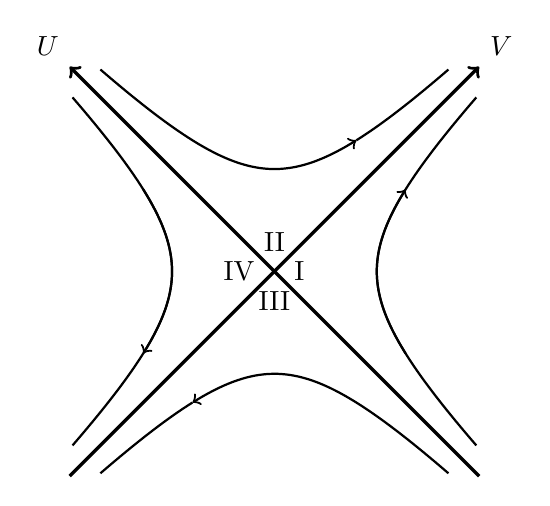
\begin{tikzpicture}[scale=1.3]
        \draw (0.1,0) node[right] {I};
        \draw (0,0.1) node[above] {II};
        \draw (0,-0.1) node[below] {III};
        \draw (-0.1,0) node[left] {IV};

        \draw[domain=-1.7:0.8,smooth,variable=\x,thick,->] plot({\x},{sqrt(1+\x*\x))});
        \draw[domain=0.8:1.7,smooth,variable=\x,thick] plot({\x},{sqrt(1+\x*\x))});

        \draw[domain=-1.7:0.8,smooth,variable=\x,thick,->] plot({-\x},{-sqrt(1+\x*\x))});
        \draw[domain=0.8:1.7,smooth,variable=\x,thick] plot({-\x},{-sqrt(1+\x*\x))});

        \draw[domain=-1.7:0.8,smooth,variable=\x,thick,->] plot({sqrt(1+\x*\x))},{\x});
        \draw[domain=-0.8:1.7,smooth,variable=\x,thick] plot({sqrt(1+\x*\x))},{\x});

        \draw[domain=-1.7:0.8,smooth,variable=\x,thick,->] plot({-sqrt(1+\x*\x))},{-\x});
        \draw[domain=-0.8:1.7,smooth,variable=\x,thick] plot({-sqrt(1+\x*\x))},{-\x});

        \draw[very thick,->] (-2,-2) -- (2,2) node[above right] {\(V\)};
        \draw[very thick,->] (2,-2) -- (-2,2) node[above left] {\(U\)};
    \end{tikzpicture}
\end{figure}

\(U=0\) and \(V=0\) are both independently fixed by \(k\). \(k=0\) on \(U=V=0\), a region known as the \emph{bifurcation 2-sphere}.

\lecture{27/01/16}
\subsection{Einstein-Rosen bridge}
Consider a constant \(t\) slice of \emph{Kruskal} spacetime. We define the coordinate \(\rho\) on this slice by
\begin{equation}
    r=\rho+M+\frac{M^2}{4\rho} \qq{such that} \rho>\frac{M}{2} \;\text{in I},\; \rho<\frac{M}{2} \; \text{in IV.}
\end{equation}
In \emph{isotropic coordinates} \((t,\rho,\theta,\phi)\), the line element is
\begin{equation}
    \dd{s}^2 = - \frac{\left(1-\frac{M}{2\rho}\right)^2}{\left(1+\frac{M}{2\rho}\right)^2} \dd{t}^2 + \left(1+\frac{M}{2\rho}\right)^4 (\dd{\rho}^2+\rho^2\dd{\Omega}^2).
\end{equation}
Note that \(\rho\to\frac{M^2}{4\rho}\) interchanges I and IV.

\begin{wrapfigure}{r}{0.4\linewidth}
    \centering
    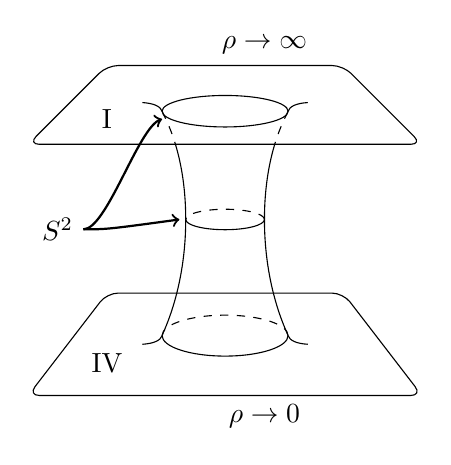
\begin{tikzpicture}
        \draw[rounded corners, shift={(0,0.08)}] (0,3) -- (5,3) -- (4,4) -- (1,4) -- cycle;
        \draw[rounded corners, shift={(0,-0.11)}] (0,0) -- (5,0) -- (4,1.3) -- (1,1.3) -- cycle;

        \draw (2.5,3.5) ellipse (0.8 and 0.2);
        \begin{scope}[shift={(0,2.125)},yscale=0.26]
            \draw (3,0) arc (0:-180:0.5);
            \draw[dashed] (3,0) arc (0:180:0.5);
        \end{scope}
        \begin{scope}[shift={(0,0.65)},yscale=0.325]
            \draw (3.3,0) arc (0:-180:0.8);
            \draw[dashed] (3.3,0) arc (0:180:0.8);
        \end{scope}
        
        \begin{scope}
            \clip[shift={(0,0.08)}] (0,3) rectangle (5,0);
            \draw (3.3,3.5) .. controls (3.28,3.44) and (3,3) .. (3,2.125)
                            .. controls (3,1.25) and (3.28,0.71) .. (3.3,0.65);
            \draw (1.7,3.5) .. controls (1.72,3.44) and (2,3) .. (2,2.125)
                            .. controls (2,1.25) and (1.72,0.71) .. (1.7,0.65);
        \end{scope}
        \begin{scope}[dashed]
            \clip[shift={(0,0.08)}] (0,3) rectangle (5,4);
            \draw (3.3,3.5) .. controls (3.28,3.44) and (3,3) .. (3,2.125)
                            .. controls (3,1.25) and (3.28,0.71) .. (3.3,0.65);
            \draw (1.7,3.5) .. controls (1.72,3.44) and (2,3) .. (2,2.125)
                            .. controls (2,1.25) and (1.72,0.71) .. (1.7,0.65);
        \end{scope}

        \draw (3.3,3.5) .. controls (3.32,3.56) and (3.4,3.6) .. (3.55,3.61);
        \draw (1.7,3.5) .. controls (1.68,3.56) and (1.6,3.6) .. (1.45,3.61);
        \draw (3.3,0.65) .. controls (3.32,0.59) and (3.4,0.55) .. (3.55,0.54);
        \draw (1.7,0.65) .. controls (1.68,0.59) and (1.6,0.55) .. (1.45,0.54);

        \node at (1,3.4) {I};
        \node at (1,0.3) {IV};

        \draw[->, thick] (0.7,2) node[left] {\(S^2\)} .. controls (1,2) and (1.4,3.3) .. (1.7,3.4);
        \draw[->, thick] (0.7,2) .. controls (1,2) .. (1.92,2.125);

        \node[above] at (3,4.1) {\(\rho\to\infty\)};
        \node[below] at (3,-0.1) {\(\rho\to0\)};
    \end{tikzpicture}
\end{wrapfigure}
On a constant \(t\) surface, the induced metric is
\begin{equation}
    \dd{s}^2 = \left(1+\frac{M}{2\rho}\right)^4 (\dd{\rho}^2+\rho^2\dd{\Omega}^2).
\end{equation}
If we take \(\rho>0\), we see that the surface is a Riemannian manifold with topology \(\RR\times S^2\). We can visualise this surface by embedding into four dimensional Euclidean space.
We have two asymptotically flat regions at \(\rho\to\infty\), \(\rho\to0\) connected by a ``throat'' with minimum radius \(r=2M\) at \(\rho = \frac{M}{2}\).

\subsection{Extendability and singularities}
\begin{defn}
    A spacetime \((\mathcal{M},g)\) is said to be \emph{extendable} if it is isometric to a proper subset of another spacetime \((\mathcal{M}',g)\), called an \emph{extension} of \((\mathcal{M},g)\).
\end{defn}
\begin{eg}
    \(r>2M\) Schwarzschild spacetime is extendable, with for example Kruskal spacetime as an extension. The isometry in question is the identity map.
    Kruskal spacetime on the other hand is inextendible, and is in fact a \emph{maximal analytic extension} of \((\mathcal{M},g)\).
\end{eg}

There are many types of singularities.
\begin{itemize}
    \item A \emph{scalar curvature singularity} is a region in which a scalar constructed from the Riemann tensor \(R_{abcd}\) blows up.
    \item More generally, a \emph{curvature singularity} is a region in which there does not exist a chart such that the components of the Riemann tensor \(R_{\mu\nu\rho\sigma}\) are finite.
    \item It is possible to have singularities which have nothing to do with the curvature tensor. For example consider \(\mathcal{M}=\RR^2\) with polar coordinates \((r,\phi)\), where we identify \(\phi \sim \phi+2\pi\), with line element given by
        \begin{equation}
            \dd{s}^2=\dd{r}^2+\lambda^2r^2\dd{\phi}^2
        \end{equation}
        for some constant \(\lambda>0\). There are two cases:
        \begin{itemize}
            \item In the case \(\lambda=1\), this is just Euclidean space, and \(r=0\) is just a coordinate singularity.
            \item If \(\lambda\ne1\), then set \(\phi'=\lambda\phi\) to obtain
                \begin{equation}
                    \dd{s}^2 = \dd{r}^2+r^2\dd{\phi'}^2.
                \end{equation}
                Locally, this is isometric to Euclidean space. It is flat, so \(R_{abcd}=0\) and there is no curvature singularity. However the range of the angular coordinate has changed; our identification has changed to \(\phi'\sim\phi+2\pi\lambda\). Consider a circle with \(r=\epsilon\). The ratio of the circumference to the radius of this circle is \(2\pi\lambda\epsilon/\epsilon=2\pi\lambda\). As we take \(\epsilon\), we would expect this ratio to approach \(2\pi\) if the geometry were locally flat at \(r=0\), but this is not the case. \(g\) is not smooth at \(r=0\). This type of singularity is called a \emph{conical singularity}.
        \end{itemize}
\end{itemize}

\begin{defn}
    \(p\in\mathcal{M}\) is a \emph{future endpoint} of a future-directed causal curve \(\gamma:(a,b)\to\mathcal{M}\) if for any neighbourhood \(\mathcal{O}\) of \(p\) there exists a \(t_0\) such that \(\gamma(t)\in\mathcal{O}\) for all \(t>t_0\). We say \(\gamma\) is \emph{future-inextendable} if it has no future endpoint.
\end{defn}

\begin{eg}
    Let \((\mathcal{M},g)\) be Minkowski space, and \(\gamma:(-\infty,0)\to\mathcal{M}\), \(\gamma(t)=(t,0,0,0)\). Then \((0,0,0,0)\) is a future end point of \(\gamma\). If however \((\mathcal{M},g)\) is Minkowski\(\setminus(0,0,0,0)\), then \(\gamma\) is future-inextendable.
\end{eg}

\begin{defn}
    A geodesic is \emph{complete} if an affine parameter extends to \(\pm\infty\). A spacetime is \emph{geodesically complete} if all inextendable geodesics are complete. If a spacetime is both inextendable and geodesically incomplete, then we say it is \emph{singular}.
\end{defn}

\section{The Initial Value Problem}
\subsection{Predictability}
\begin{defn}
    A \emph{partial Cauchy surface} \(\Sigma\) is a hypersurface for which no two points are connected by a causal curve in \(\mathcal{M}\).
\end{defn}
\begin{defn}
    The \emph{future domain of dependence} of \(\Sigma\) is the set 
    \begin{equation}
        D^+(\Sigma) = \{p\in\mathcal{M}\;\st\;\text{every past-inextendible causal curve through \(p\) intersects \(\Sigma\)}\}.
    \end{equation}
    We define the \emph{past domain of dependence} \(D^-(\Sigma)\) in a similar way. The \emph{domain of dependence} is \(D(\Sigma) = D(\Sigma^+)\cup D(\Sigma^-)\).
\end{defn}

A causal geodesic in \(D(\Sigma)\) is uniquely determined by its velocity at \(q\in\Sigma\) (this is because the geodesic equation is a hyperbolic PDE).

\begin{eg}
    Consider 2d Minkowski space, and the surface \(\Sigma = \{(0,x)\st x>0\}\). Then \(D^+(\Sigma)= \{(t,x)\st 0 \le t < x\}\), \(D^-(\Sigma)= \{(t,x)\st -x < t \le 0\}\).
\end{eg}

\begin{defn}
    \((\mathcal{M},g)\) is called \emph{globally hyperbolic} if it contains a \emph{Cauchy surface} i.e.\ a partial Cauchy surface whose domain of dependence is all of \(\mathcal{M}\).
\end{defn}

\begin{eg}
    Minkowsi spacetime is globally hyperbolic (for instance \(t\) constant is a Cauchy surface). Kruskal spacetime is globally hyperbolic (for instance \(U+V\) constant is a Cauchy surface).

    2d Minkowski spacetime with \((0,0)\) removed is \emph{not} globally hyperbolic.
\end{eg}

\begin{theorem}
    Suppose \((\mathcal{M},g)\) is a globally hyperbolic spacetime. Then:
    \begin{enumerate}
        \item There exists a \emph{global time function} i.e.\ a map \(t:\mathcal{M}\to\RR\) such that \((\dd{t})^a\) is future-directed and timelike.
        \item \(t\) constant surfaces are Cauchy and all have the same topology \(\Sigma\).
        \item \(\mathcal{M} = \RR\times\Sigma\).
    \end{enumerate}
\end{theorem}

Exercise: show \(U+V\) is a global time function for Kruskal spacetime. \(U+V = 0\) is an Einstein-Rosen bridge, so \(\Sigma = \RR \times S^2\) and \(\mathcal{M} = \RR^2\times S^2\).


\begin{wrapfigure}{r}{0.4\linewidth}
    \centering
    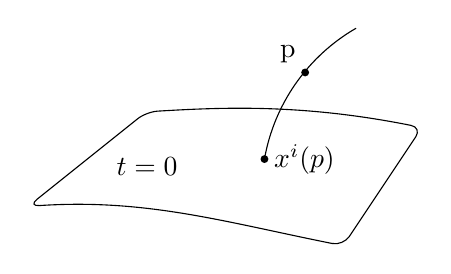
\begin{tikzpicture}
        \draw[rounded corners] (0,0) .. controls (1.5,0.1) and (2.5,-0.2) .. (4,-0.5)
                                     -- (5, 1)
                                     .. controls (3.5, 1.3) and (2.5,1.26) .. (1.5,1.2)
                                     -- cycle;
        \draw (3,0.6) arc (170:120:2.4);
        \fill (3,0.6) circle (0.05) node[right] {\(x^i(p)\)};
        \fill (3.517,1.7) circle (0.05) node [above left] {p};
        \node[right] at (1,0.5) {\(t=0\)};
    \end{tikzpicture}
\end{wrapfigure}
If we have a time function \(t\), we will often carry out a \emph{3+1 split} to obtain a set of local coordinates. Suppose we have coordinates \(x^i\) on the surface \(t=0\), and a timelike vector field \(T^a\).
For a point \(p\) near \(t=0\), we let \(x_i(p)\) be the coordinate of the point where the integral curve of \(T^a\) through \(p\) intersects \(t=0\). Thus we have a coordinate chart \(t,x^i\). In these coordinates, the metric is given by
\begin{equation}
    \dd{s}^2 = -N(t,x)^2\dd{t}^2 + h_{ij}(t,x)(\dd{x^i} + N^i(t,x)\dd{t})(\dd{x^j} + N^j(t,x)\dd{t}),
\end{equation}
where \(N\) and \(N^i\) are known as the \emph{lapse function} and \emph{shift vector} respectively, and \(h_{ij}\) is the metric on a constant \(t\) surface.

\subsection{Initial value problem in GR}
\lecture{29/01/16}
We can view the Einstein equations as an initial value problem. We are given \(\Sigma\), a 3d Riemannian manifold with metric \(h_{ab}\) and extrinsic curvature \(K_{ab}\). In addition we have the \emph{Hamiltonian constraint}
\begin{equation}
    R' - K^{ab}K_{ab} + K^2 = 16\pi\rho,
\end{equation}
where \(R'\) is the Ricci scalar of \(h\), \(K=K\indices{_a^a}\) and \(\rho = T_{ab}n^an^b\) (with \(n\) a unit normal to \(\Sigma\)), and the \emph{momentum constraint}
\begin{equation}
    D_bK\indices{^b_a} - D_aK = 8\pi h\indices{_a^b}T_{bc}n^c,
\end{equation}
where \(D_b\) is the Levi-Civita connection with regard to \(h\).

\begin{theorem}[Choquet-Bruhat and Geroch 1969]
    Given initial data satisfying vacuum constraints (i.e.\ the right hand sides of the above equal to 0), there exists a unique (up to diffeomorphism) spacetime \(\mathcal{M},g\), known as the \emph{maximal Cauchy development} of \(\Sigma, h_{ab}, K_{ab}\), such that the following are satisfied:
    \begin{enumerate}
        \item \((\mathcal{M},g)\) obeys the vacuum Einstein equations.
        \item \((\mathcal{M},g)\) is globally hyperbolic with Cauchy surface \(\Sigma\).
        \item The induced metric and extrinsic curvature of \(\Sigma\) are \(h_{ab}\) and \(K_{ab}\) respectively.
        \item Any other spacetime obeying 1-3 is isometric to a subset of \((\mathcal{M},g)\).
    \end{enumerate}
\end{theorem}
Note that \((\mathcal{M},g)\) may be extendable, but the solution will be non-unique outside of \(D(\Sigma)\).
\begin{eg}
    Consider \(\Sigma = \{(x,y,z)\st x>0\}\), \(h_{\mu\nu} = \delta_{\mu\nu}\), \(K_{\mu\nu} = 0\). Then \((\mathcal{M},g)\) is the region of Minkowski spacetime with \(|t|<x\), and this is clearly extendable.
\end{eg}
In the preceding example, \((\mathcal{M},g)\) was extendable because \((\Sigma, h_{ab})\) was extendable, but this need not be the case.
\begin{eg}
    Consider \(M<0\) Schwarzschild. The metric is
    \begin{equation}
        \dd{s}^2 = - \left(1+\frac{2|M|}{r}\right)\dd{t}^2 + \left(1+\frac{2|M|}{r}\right)^{-1}\dd{r}^2 + r^2\dd{\Omega}^2.
    \end{equation}
    There is a curvature singularity at \(r=0\) but, unlike the positive mass case, there is no event horizon. We choose the initial data \((\Sigma,h_{ab},K_{ab})\) to be that given by the surface \(t=0\); this is inextendable (but not geodesically complete since it is singular at \(r=0\)). For outgoing radial null geodesics at small \(r\), we have 
    \begin{equation}
        \pdv{t}{r} = \left(1+\frac{2|M|}{r}\right)^{-1} \approx \frac{r}{2|M|},
    \end{equation}
    so we can write \(t \approx t_0 + \frac{r^2}{4|M|}\). If \(t_0>0\) then the geodesic never intersects \(\Sigma\), so \(\Sigma\) is not a Cauchy surface for \(\mathcal{M}\). The boundary of \(D(\Sigma)\) is given by those geodesics with \(t_0=0\).
    \begin{figure}[H]
        \centering
        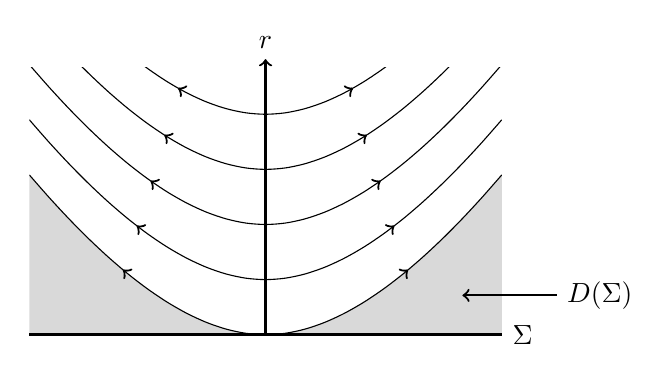
\begin{tikzpicture}
            \fill[gray!30, domain=-3:3,smooth,variable=\x] plot({\x},{1.5*abs(\x)*(1-exp(-0.2*abs(\x)))}) -- (3,0) -- (-3,0) -- cycle;

            \begin{scope}
                \clip (-3,0) rectangle (3,3.4);
                \foreach \tz in {0,0.7,1.4,2.1,2.8}
                {
                    \draw[domain=-3:3,smooth,variable=\x] plot({\x},{\tz+1.5*abs(\x)*(1-exp(-0.2*abs(\x)))});
                    \draw[thick, ->] (1.8-\tz/4,{\tz+1.5*(1.8-\tz/4)*(1-exp(-0.2*(1.8-\tz/4)))}) 
                        -- (1.81-\tz/4,{\tz+1.5*(1.81-\tz/4)*(1-exp(-0.2*(1.81-\tz/4)))});
                    \draw[thick, ->] (-1.8+\tz/4,{\tz+1.5*(1.8-\tz/4)*(1-exp(-0.2*(1.8-\tz/4)))}) 
                        -- (-1.81+\tz/4,{\tz+1.5*(1.81-\tz/4)*(1-exp(-0.2*(1.81-\tz/4)))});
                }
            \end{scope}

            \draw[thick,->] (0,0) -- (0,3.5) node[above] {\(r\)};
            \draw[very thick] (-3,0) -- (3,0) node[right] {\(\Sigma\)};

            \draw[thick,<-] (2.5,0.5) -- (3.7,0.5) node [right] {\(D(\Sigma)\)};
        \end{tikzpicture}
    \end{figure}
    The solution outside of \(D(\Sigma)\) is \emph{not} determined by the data on \(\Sigma\); in particular, it need not be the negative mass Schwarzschild that we started with.
\end{eg}
This time, the maximal development was extendable because the initial data was singular, but again this is not necessary.
\begin{eg}
    Consider 4d Minkowski spacetime, and start with data on the surface \(\Sigma = \{-t^2+x^2+y^2+z^2 = -1, t < 0\}\). This is one sheet of a hyperboloid. The maximal development of \(\Sigma\) is the interior of the past lightcone of the origin, and this is extendable.
    \begin{figure}[H]
        \centering
        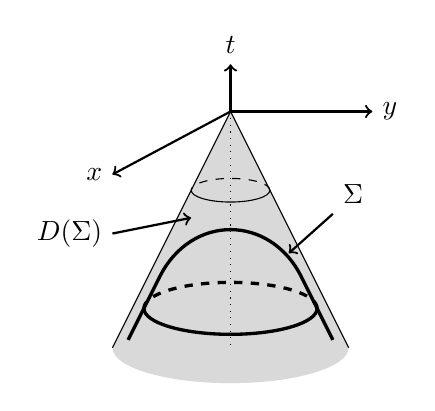
\begin{tikzpicture}
            \fill[gray!30,yscale=0.3] (0,0) -- (1.5,-10) arc (0:-180:1.5) -- cycle;

            \draw[thick,->] (0,0) -- (0,0.6) node[above] {\(t\)};
            \draw[thick,->] (0,0) -- (1.8,0) node[right] {\(y\)};
            \draw[thick,->] (0,0) -- (-1.5,-0.8) node[left] {\(x\)};

            \draw[dotted] (0,0) -- (0,-3);

            \draw (0,0) -- (1.5,-3);
            \draw (0,0) -- (-1.5,-3);
            \draw[shift={(0.5,-1)},yscale=0.3] (0,0) arc (0:-180:0.5);
            \draw[shift={(0.5,-1)},yscale=0.3, dashed] (0,0) arc (0:180:0.5);

            \draw[very thick] (1.3,-2.9) -- (0.9,-2.1)
                .. controls (0.5,-1.3) and (-0.5,-1.3)
                .. (-0.9,-2.1) -- (-1.3,-2.9);

            \draw[very thick, shift={(1.1,-2.5)},yscale=0.3] (0,0) arc (0:-180:1.1);
            \draw[very thick, shift={(1.1,-2.5)},yscale=0.3, dashed] (0,0) arc (0:180:1.1);

            \draw[thick, <-] (0.74,-1.8) -- (1.3,-1.3) node[above right] {\(\Sigma\)};
            \draw[thick, <-] (-0.5, -1.35) -- (-1.5,-1.55) node [left] {\(D(\Sigma)\)};
        \end{tikzpicture}
    \end{figure}
\end{eg}
Now, the maximal development is extendible because the initial data is ``asymptotically null''. To avoid this problem, we will use asymptotically flat initial data.

\begin{defn}
    \((\Sigma,h_{ab},K_{ab})\) is an \emph{asymptotically flat end} if:
    \begin{itemize}
        \item \(\Sigma\) is diffeomorphic to \(\RR^3\setminus B\) where \(B\) is a closed ball centred on the origin in \(\RR^3\).
        \item If we pull back \(\RR^3\) coordinates to give coordinates \(x^i\) on \(\Sigma\), then the metric is \(h_{ij} = \delta_{ij} + O(1/r)\) and the extrinsic curvature is \(K_{ij} = O(1/r^2)\).
        \item \(h_{ij,k} = O(1/r^2)\) etc.
    \end{itemize}
\end{defn}

\begin{defn}
    A set of initial data is said to be \emph{asymptotically flat with \(N\) ends} if it is a union of a compact set with \(N\) asymptotically flat ends.
\end{defn}

\begin{eg}
    Consider \(M>0\) Schwarzschild spacetime. \(\Sigma = \{t = \text{constant}, r>2M\}\) is an asymptotically flat end. \(\Sigma\) is part of an Einstein-Rosen bridge, which is asymptotically flat with 2 ends (in fact it is the union of two copies of \(\Sigma\) and the bifurcation two-sphere at \(r=2M\)).
\end{eg}

\subsection{Strong cosmic censorship}
The strong cosmic censorship conjecture (by Penrose) is the following:
\begin{quote}
    Given vacuum initial data \((\Sigma,h_{ab},K_{ab})\) that is geodesically complete and asymptotically flat, then  generically the maximal Cauchy development is inextendable.
\end{quote}
The conjecture has been shown to be true for nearly flat data, but there are non-generic counterexamples.

\section{The Singularity Theorem}
\subsection{Null hypersurfaces}
\lecture{01/02/16}
\begin{defn}
    A \emph{null hypersurface} is a hupersurface \(\mathcal{N}\) whose normal \(n\) is everywhere null.
\end{defn}
\begin{eg}
    Consider a constant \(r\) surface in Schwarzschild spacetime in ingoing Eddington-Finklestein coordinates. The metric is
    \begin{equation}
        g^{\mu\nu} = 
        \begin{pmatrix}
            0 & 1 & 0 & 0 \\
            1 & 1 - \frac{2M}{r} & 0 & 0 \\
            0 & 0 & \frac{1}{r^2} & 0 \\
            0 & 0 & 0 & \frac{1}{r^2\sin^2\theta}
        \end{pmatrix}.
    \end{equation}
    The normal 1-form is \(n=\dd{r}\), and we have \(n^2 = g^{\mu\nu}n_\mu n_\nu = g^{rr} = 1 - \frac{2M}{r}\), so \(r=2M\) is a null hypersurface.
\end{eg}

Note that iff \(X^a\) is tangent to \(\mathcal{N}\), then either \(X^a\) is spacelike or it is parallel to \(n^a\). Thus \(n^a\) is tangent to \(\mathcal{N}\) and in particular the integral curves of \(n^a\) lie within \(\mathcal{N}\).

\begin{lemma}
    The integral curves of \(n^a\) are null geodesics (they are referred to as the \emph{generators} of \(\mathcal{N}\)).
\end{lemma}
\begin{proof}
    Define \(\mathcal{N}\) by \(f = \text{constant}\) for some function \(f\). We have \(\dd{f}\ne 0\) on \(\mathcal{N}\) and \(n=h\dd{f}\) for some \(h\). Let \(N=\dd{f}\). The integral curves of \(n\) and \(N\) are the same up to reparametrisation, so we focus on \(N\). Since \(N\) is null, we have \(N_aN^a=0\) on \(\mathcal{N}\), and so \(\dd{(N_aN^a)}\) is normal to \(\mathcal{N}\). Thus, \(\nabla_a(N^bN_a) = 2\alpha N_a\) for some \(\alpha\) on \(\mathcal{N}\). The left hand side is
    \begin{equation}
        2N^b\nabla_a N_b = 2N^b \nabla_a\nabla_b f = 2N^b\nabla_b\nabla_a f = 2N^b\nabla_bN_a.
    \end{equation}
    Hence on \(\mathcal{N}\), \(N_a\) satisfies the geodesic equation \(N^b\nabla_b N_a = \alpha N_a\).
\end{proof}

\begin{eg}
    Consider Kruskal spacetime with coordinates \((U,V,\theta,\phi)\). \(N=\dd{U}\) is null everywhere, so we have a family of null hypersurfaces \(U = \text{constant}\). In this case, we have \(N^b\nabla_b N_a = \frac{1}{2}\nabla_a(N^2) = 0\), so \(N^a\) is tangent to affinely parametrised geodesics. It is easy to show that \(N^a = - \frac{r}{16M^3}e^{r/2M} \left(\pdv{V}\right)^a\), so if we let \(\mathcal{N}=\{U=0\}\) then \(V\) is an affine parameter for generators of \(\mathcal{N}\), and similarly \(U\) is an affine parameter for generators of \(\{V=0\}\).
\end{eg}

\subsection{Geodesic deviation}
\begin{defn}
    A \emph{1-parameter family} of geodesics is a function \(\gamma:I\times I'\to\mathcal{M}\) where \(I,I'\) are open intervals in \(\RR\), such that \(\lambda\mapsto\gamma(s,\lambda)\) is a geodesic with affine parameter \(\lambda\) and \((s,\lambda)\mapsto\gamma(s,\lambda)\) is smooth and 1-to-1 with a smooth inverse.
\end{defn}

\begin{wrapfigure}{l}{0.3\linewidth}
    \centering
    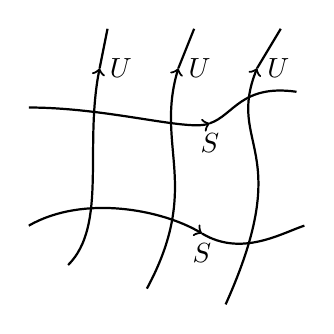
\begin{tikzpicture}
        \draw[thick, ->] (0,0) .. controls (0.5, 0.5) and (0.2,1.5) .. (0.4,2.5) node[right] {\(U\)};
        \draw[thick] (0.4,2.5) -- (0.5,3);
        \draw[thick, ->] (1,-0.3) .. controls (1.7, 1) and (1.1,1.5) .. (1.4,2.5) node[right] {\(U\)};
        \draw[thick] (1.4,2.5) -- (1.6,3);
        \draw[thick, ->] (2,-0.5) .. controls (2.9, 1.5) and (2,1.5) .. (2.4,2.5) node[right] {\(U\)};
        \draw[thick] (2.4,2.5) -- (2.7,3);

        \draw[thick, ->] (-0.5,2) .. controls (0.5, 2) and (1.5,1.7) .. (1.8,1.8) node[below] {\(S\)};
        \draw[thick] (1.8,1.8) .. controls (2.1,1.9) and (2.2,2.3) .. (2.9,2.2);
        \draw[thick, ->] (-0.5,0.5) .. controls (0.2, 0.9) and (1.2,0.7) .. (1.7,0.4) node[below] {\(S\)};
        \draw[thick] (1.7,0.4) .. controls (2.2,0.1) and (2.7,0.4) .. (3,0.5);
    \end{tikzpicture}
\end{wrapfigure}
Let \(\gamma(s,\lambda)\) take coordinates \(x^\mu(s,\lambda)\); we define the vector fields
\begin{equation}
    S^\mu = \pdv{x^\mu}{s} \qq{and} U^\mu = \pdv{x^\mu}{\lambda}.
\end{equation}
We also define the \emph{deviation vectors} (?) from the coordinates \(s,\lambda\) on the image of \(\gamma\),
\begin{equation}
    S = \pdv{s} \qq{and} U = \pdv{\lambda}.
\end{equation}

We have \([S,U] = 0\), so we can write \(U^b\nabla_bS^a = S^b\nabla_bU^a\), and thus obtain the \emph{geodesic deviation equation}
\begin{equation}
    U^c\nabla_c(U^b\nabla_bS^a)=R\indices{^a_b_c_d}U^bU^cS^d.
\end{equation}
A solution \(S^a\) to this equation along \(\gamma\) is called a \emph{Jacobi field}.

\subsection{Geodesic congruences}
\begin{defn}
    Let \(\mathcal{U}\in\mathcal{M}\) be open. A \emph{geodesic congruence} is a family of geodesics such that exactly one geodesic passes through each \(p\in\mathcal{U}\).
\end{defn}
Let \(U^a\) be the tangent vector of a geodesic congruence, normalised such that \(U^2 = -1\) if timelike, \(0\) if null, and \(1\) if spacelike. We define the \emph{velocity gradient} \(B\indices{^a_b} = \nabla_bU^a\). By the above we have \(U^b\nabla_bS^a = B\indices{^a_b}S^b\). It is easy to see that \(U_aB\indices{^a_b} = 0 = B\indices{^a_b}U^b\). We also have
\begin{equation}
    U\vdot\nabla(U\vdot S) = \underbrace{(U\vdot\nabla U^a)}_{=0}S_a + U^a U\vdot\nabla S_a = \underbrace{U^aB_{ab}}_{=0}S^b = 0,
\end{equation}
so \(U\vdot S\) is constant along any geodesic in the congruence.

Suppose we redefine our affine parameter \(\lambda \to \lambda' = \lambda - a(s)\). We have \(S'^a = S^a + \dv{a}{s}U^a\). \(S^a\) and \(S'^a\) point to the same geodesics, so we have a kind of gauge freedom here. Note that \(U\vdot S' = U\vdot S + \dv{a}{s}U^2\), so in the spacelike and timelike cases, we can choose \(a(s)\) such that \(U\vdot S=0\) at \(\lambda = 0\), and hence everywhere.

\subsection{Null geodesic congruences}
Things are less easy if \(U\) is null. Pick some spacelike hypersurface \(\Sigma\) that is tranverse to \(U\) (i.e.\ not tangent). Pick a vector field \(N^a\) such that \(N^2=0\) and \(N\vdot U = -1\) on \(\Sigma\), and additionally \(U\vdot\nabla N^a = 0\). It can be shown that this implies that \(N^2 = 0\) and \(N\vdot U=-1\) everywhere. Now write
\begin{equation}
    S^a = \alpha U^a + \beta N^a + \hat{S}^a
\end{equation}
where \(U\vdot \hat{S} = N\vdot\hat{S} = 0\) (this means that \(\hat{S}^a\) is either spacelike or zero). We have \(U\vdot S = -\beta\), so \(\beta\) is constant along each geodesic. Note that \(\alpha U^a + \hat{S}^a\) is orthogonal to \(U^a\) and \(\beta N^a\) is parallely transported along \(U^a\).

\begin{eg}
    Consider a null hypersurface \(\mathcal{N}\) and pick a congruence containing the generators of \(\mathcal{N}\). For a 1-parameter family of generators, we have \(S^a\) tangent to \(\mathcal{N}\), and so \(\beta = -U\vdot S = 0\).
\end{eg}

We can write \(\hat{S}^a = P\indices{^a_b}S^b\) where \(P\indices{^a_b} = \delta^a_b = N^aU_b + U^aN_b\). \(P\indices{^a_b}\) is a projection (\(P\indices{^a_b}P\indices{^b_c} = P\indices{^a_c}\)) onto \(T_\perp = \{\text{vectors \(\perp\) to \(U^a,N^a\)}\} \subset T_p(\mathcal{M})\), a 2d space.  We have \(U\vdot\nabla P\indices{^a_b} = 0\).

\begin{lemma}
    If \(U\vdot S = 0\), then \(U\vdot\nabla\hat{S}^a = \hat{B}\indices{^a_b}\hat{S}^b\), where \(\hat{B}\indices{^a_b} = P\indices{^a_c}B\indices{^c_d}P\indices{^d_b}\).
\end{lemma}
\begin{proof}
    We have:
    \begin{align}
        U\vdot\nabla\hat{S}^a &= U\vdot\nabla(P\indices{^a_c}S^c) \\
                              &= P\indices{^a_c}U\vdot\nabla S^c \\
                              &= P\indices{^a_c}B\indices{^c_d}S^d \\
                              &= P\indices{^a_c}B\indices{^c_d}P\indices{^d_e}S^e \quad \text{(using \(B\vdot U=U\vdot S=0\))} \\
                              &= \underbrace{P\indices{^a_c}B\indices{^c_d}P\indices{^d_b}}_{=\hat{B}\indices{^a_b}}\underbrace{P\indices{^b_e}S^e}_{=\hat{S}^b} \quad \text{(since \(P = P^2\))} \qedhere
    \end{align}
\end{proof}

\subsection{Expansion, rotation and shear}
\lecture{03/02/16}
\begin{defn}
    \emph{Expansion} \(\theta\), \emph{rotation} \(\hat{\omega}_{ab}\) and \emph{shear} \(\hat{\sigma}_{ab}\) are defined in the following way:
    \begin{equation}
        \theta = \hat{B}\indices{^a_a} \quad \hat{\omega} = \hat{B}_{[ab]} \quad \hat{\sigma}_{ab} = \hat{B}_{(ab)} - \frac{1}{2}P_{ab}\theta
    \end{equation}
\end{defn}
We have \(\hat{B}\indices{^a_b} = \frac{1}{2}\theta P\indices{^a_b} + \hat{\sigma}\indices{^a_b} + \hat{\omega}\indices{^a_b}\), and it can be shown that \(\theta = g^{ab}B_{ab} = \nabla_a U^a\).

\begin{lemma}
    If a congruence contains the generators of a null hypersurface \(\mathcal{N}\), then \(\hat{\omega}=0\) on \(\mathcal{N}\). Conversely, if \(\hat{\omega}=0\) then \(U^a\) is everywhere hypersurface orthogonal.
\end{lemma}
\begin{proof}
    Since \(B\vdot U = U\vdot B = 0\), we can write 
    \begin{equation}
        \hat{B}\indices{^b_c} = B\indices{^b_c} + U^bN_dB\indices{^d_c} + U_cB\indices{^b_d}N^d + U^bU_c N_dB\indices{^d_e}N^e.
    \end{equation}
    We have
    \begin{equation}
        U_{[a}\hat{\omega}_{bc]} = U_{[a}\hat{B}_{bc]} 
                                 = U_{[a}B_{bc]} 
                                 = U_{[a}\nabla_cU_{b]} 
                                 = - \frac{1}{6} (U\wedge\dd{U})_{abc},
    \end{equation}
    so since \(U^a\) is orthogonal to \(\mathcal{N}\) and hence \(U\wedge\dd{U} = 0\) on \(\mathcal{M}\), we can conclude
    \begin{equation}
        0 = \left. U_{[a}\hat{\omega}_{bc]} \right|_{\mathcal{N}} = \left.\frac{1}{3}(U_a\hat{\omega}_{bc} + U_b\hat{\omega}_{ca} + U_c\hat{\omega}_{ab}) \right|_{\mathcal{N}}.
    \end{equation}
    Contracting with \(N^a\), we see that \(\hat{\omega}_{bc} = 0\) on \(\mathcal{N}\) as required.

    For the converse, we have \(\hat{\omega} = 0 \implies U\wedge\dd{U}=0\), which by Frobenius' theorem implies \(U\) is hypersurface orthogonal.
\end{proof}

Consider geodesics in \(\mathcal{N}\) with tangent vector \(S^a\). By foliating \(\mathcal{N}\) into a family of constant \(\lambda\) surfaces, we can visualise how expansion and shear act on these geodesics.
\begin{figure}[H]
    \centering
    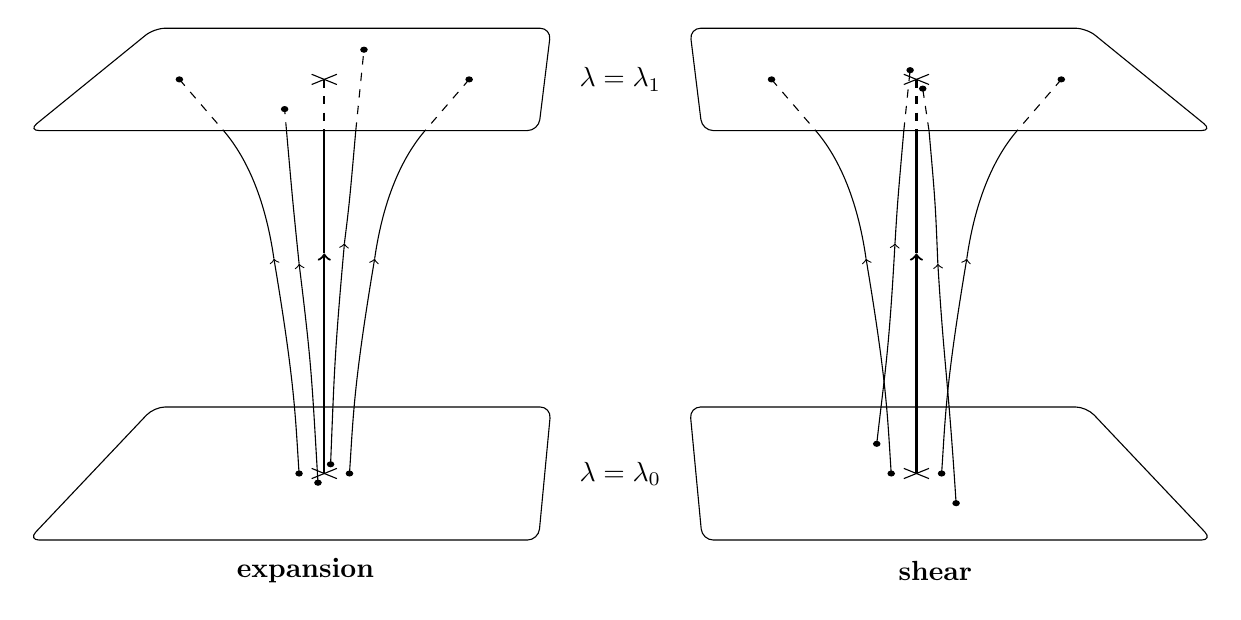
\begin{tikzpicture}[xscale=1.6,yscale=1.3]
        \begin{scope}[xscale=-1]
            \draw[rounded corners] (0.65,4) -- (4.7,4) -- (3.7,5) -- (0.55,5) -- cycle;
            \draw[rounded corners] (0.65,0) -- (4.7,0) -- (3.7,1.3) -- (0.55,1.3) -- cycle;

            \begin{scope}[shift={(4.7,0)},xscale=-1]
                \draw[->] (2.55,0.65) .. controls (2.58,1.2) and (2.58,1.5) .. (2.75,2.75);
                \draw (2.75,2.75) .. controls (2.82,3.35) and (2.975,3.75) .. (3.15,4);
                \draw[dashed] (3.5,4.5) -- (3.15,4);
                \fill (2.55,0.65) circle (0.03);
                \fill (3.5,4.5) circle (0.03);
            \end{scope}

            \draw[->] (2.55,0.65) .. controls (2.58,1.2) and (2.58,1.5) .. (2.75,2.75);
            \draw (2.75,2.75) .. controls (2.82,3.35) and (2.975,3.75) .. (3.15,4);
            \draw[dashed] (3.5,4.5) -- (3.15,4);
            \fill (2.55,0.65) circle (0.03);
            \fill (3.5,4.5) circle (0.03);

            \draw[->] (2.4,0.56) .. controls (2.45,1.6) and (2.45,1.7) .. (2.55,2.7);
            \draw (2.55,2.7) .. controls (2.6,3.3) .. (2.65, 4);
            \draw[dashed] (2.65,4) -- (2.665,4.21);
            \fill (2.4,0.56) circle (0.03);
            \fill (2.665,4.21) circle (0.03);

            \draw[->] (2.3,0.74) .. controls (2.27,1.65) and (2.27,1.8) .. (2.19,2.9);
            \draw (2.19,2.9) .. controls (2.15,3.3) .. (2.1, 4);
            \draw[dashed] (2.1,4) -- (2.035,4.79);
            \fill (2.3,0.74) circle (0.03);
            \fill (2.035,4.79) circle (0.03);

            \draw[thick,->] (2.35,0.65) -- (2.35,2.8);
            \draw[thick] (2.35,2.8) -- (2.35,4);
            \draw[thick,dashed] (2.35,4.5) -- (2.35,4);
            \begin{scope}[shift={(2.35,4.5)},yscale=0.5]
                \draw (-0.1,-0.1) -- (0.1,0.1);
                \draw (0.1,-0.1) -- (-0.1,0.1);
            \end{scope}
            \begin{scope}[shift={(2.35,0.65)},yscale=0.5]
                \draw (-0.1,-0.1) -- (0.1,0.1);
                \draw (0.1,-0.1) -- (-0.1,0.1);
            \end{scope}

            \node at (2.5,-0.3) {\bfseries expansion};
        \end{scope}
        \draw[rounded corners] (0.65,4) -- (4.7,4) -- (3.7,5) -- (0.55,5) -- cycle;
        \draw[rounded corners] (0.65,0) -- (4.7,0) -- (3.7,1.3) -- (0.55,1.3) -- cycle;

        \begin{scope}[shift={(4.7,0)},xscale=-1]
            \draw[->] (2.55,0.65) .. controls (2.58,1.2) and (2.58,1.5) .. (2.75,2.75);
            \draw (2.75,2.75) .. controls (2.82,3.35) and (2.975,3.75) .. (3.15,4);
            \draw[dashed] (3.5,4.5) -- (3.15,4);
            \fill (2.55,0.65) circle (0.03);
            \fill (3.5,4.5) circle (0.03);
        \end{scope}

        \draw[->] (2.55,0.65) .. controls (2.58,1.2) and (2.58,1.5) .. (2.75,2.75);
        \draw (2.75,2.75) .. controls (2.82,3.35) and (2.975,3.75) .. (3.15,4);
        \draw[dashed] (3.5,4.5) -- (3.15,4);
        \fill (2.55,0.65) circle (0.03);
        \fill (3.5,4.5) circle (0.03);

        \draw[->] (2.665,0.36) .. controls (2.6,1.6) and (2.57,1.7) .. (2.52,2.7);
        \draw (2.52,2.7) .. controls (2.5,3.3) .. (2.45, 4);
        \draw[dashed] (2.45,4) -- (2.4,4.41);
        \fill (2.665,0.36) circle (0.03);
        \fill (2.4,4.41) circle (0.03);

        \draw[->] (2.035,0.94) .. controls (2.1,1.65) and (2.13,1.8) .. (2.18,2.9);
        \draw (2.18,2.9) .. controls (2.2,3.3) .. (2.25, 4);
        \draw[dashed] (2.25,4) -- (2.3,4.59);
        \fill (2.035,0.94) circle (0.03);
        \fill (2.3,4.59) circle (0.03);

        \draw[thick,->] (2.35,0.65) -- (2.35,2.8);
        \draw[thick] (2.35,2.8) -- (2.35,4);
        \draw[thick,dashed] (2.35,4.5) -- (2.35,4);
        \begin{scope}[shift={(2.35,4.5)},yscale=0.5]
            \draw (-0.1,-0.1) -- (0.1,0.1);
            \draw (0.1,-0.1) -- (-0.1,0.1);
        \end{scope}
        \begin{scope}[shift={(2.35,0.65)},yscale=0.5]
            \draw (-0.1,-0.1) -- (0.1,0.1);
            \draw (0.1,-0.1) -- (-0.1,0.1);
        \end{scope}

        \node at (2.5,-0.3) {\bfseries shear};

        \node at (0,0.65) {\(\lambda=\lambda_0\)};
        \node at (0,4.5) {\(\lambda=\lambda_1\)};
    \end{tikzpicture}
\end{figure}
With expansion, geodesics move apart from one another for positive \(\theta\), and closer together for negative \(\theta\). If there is a shear, then geodesics move closer together in one direction, but further apart in the other.

\subsection{Gaussian null coordinates}
We can define a vector field \(V\) on \(\mathcal{N}\) by
\begin{equation}
    V^2 = 0, \quad V\vdot U = 1 \qq{and} V\vdot\pdv{y^i} = 0.
\end{equation}

\begin{wrapfigure}{r}{0.5\linewidth}
    \centering
    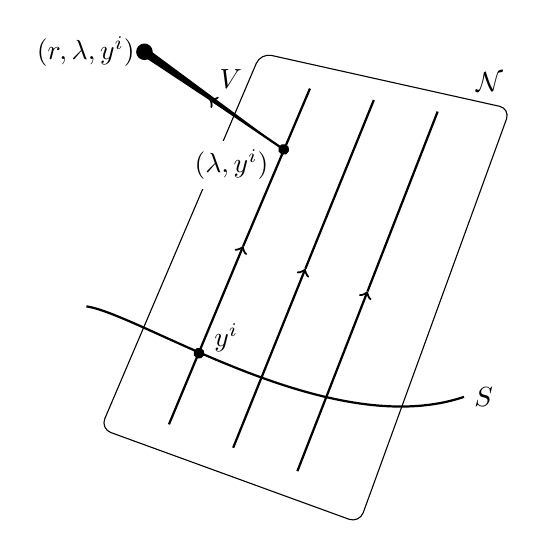
\begin{tikzpicture}[rotate=-20,scale=1.4]
        \node[above] at (2.3,4) {\(\mathcal{N}\)};
        \draw[rounded corners] (0,0) -- (2.5,0) -- (2.5,4) -- (0.2,3.7) -- cycle;
        \node[left, fill=white] at (0.695,2.8) {\((\lambda,y^i)\)};
        \draw[thick,->] (0.57,0.25) -- (0.65,2);
        \draw[thick] (0.65,2) -- (0.73,3.55);
        \draw[thick,->] (1.19,0.25) -- (1.25,2);
        \draw[thick] (1.25,2) -- (1.31,3.65);
        \draw[thick,->] (1.81,0.25) -- (1.85,2);
        \draw[thick] (1.85,2) -- (1.89,3.75);
        \draw[thick] (-0.5,1) .. controls (0,1.1) and (2,0.6) .. (3,1.4) node[right] {\(S\)};
        \fill (0.605,0.95) circle (0.05);
        \node[right] at (0.605,1.1) {\(y^i\)};
        \fill (0.695,2.95) circle (0.05);
        \draw[thick,->] (0.695,2.95) -- (-0.095,3.15) node[above right] {\(V\)};
        \fill (0.695,2.95) -- (-0.79,3.39) -- (-0.8,3.31) -- cycle;
        \fill (-0.795,3.35) circle (0.075) node[left] {\((r,\lambda,y^i)\)};
    \end{tikzpicture}
\end{wrapfigure}
To construct \emph{Gaussian null coordinates} near \(\mathcal{N}\), we assign the coordinates \((r,\lambda,y^i)\) to a point affine parameter distance \(r\) along a null geodesic starting at \((\lambda,y^i)\in\mathcal{N}\) with tangent \(V^a\) there.

Recall that \(U=\pdv{\lambda}\), so \(V=\pdv{r}\) is tangent to affinely parametrised null geodesics, so \(g_{rr} = 0\). Exercise: the geodesic equation reduces to \(g_{r\mu,r} = 0\). Therefore we have \(g_{r\lambda} = g_{r\lambda}|_{r=0} = U\vdot V|_{\mathcal{N}} = 1\) and \(g_{ri} = g_{ri}|_{r=0} = \left.V\vdot \pdv{y^i}\right|_{\mathcal{N}} = 0\). Also, since \(g_{\lambda\lambda}|_{r=0} = U^2|_{\mathcal{N}} = 0\) we have \(g_{\lambda\lambda} = rF\), and similarly since \(g_{\lambda i} |_{r=0} = \left. U\vdot\pdv{y^i}\right|_{\mathcal{N}} = 0\) we have \(g_{\lambda i} = r h_i\), where \(F\) and \(h_i\) are some smooth functions. Hence we have the following line element:
\begin{equation}
    \dd{s}^2 = 2\dd{r}\dd{\lambda} + rF\dd{\lambda}^2 + 2rh_i\dd{\lambda}\dd{y^i} + h_{ij}\dd{y^i}\dd{y^j}
\end{equation}
The induced line element on \(\mathcal{N}\) is therefore
\begin{equation}
    \dd{s}^2|_{\mathcal{N}} = 2\dd{r}\dd{\lambda} + h_{ij}\dd{y^i}\dd{y^j}.
\end{equation}
Using this metric, we can move the index downstairs on \(U^\mu|_{\mathcal{N}} = (0,1,0,0)\) to obtain \(U_\mu|_{\mathcal{N}} = (1,0,0,0)\), and hence from \(U\vdot B = B\vdot U = 0\), we have \(B\indices{^r_\mu} = B\indices{^\mu_\lambda} = 0\). Also
\begin{align}
    \theta = B\indices{^\mu_\mu} = B\indices{^i_i} &= \nabla_i U^i = \partial_i U^i + \Gamma^i_{i\mu}U^\mu \\
       &= \Gamma^i_{i\mu} = \frac{1}{2}(g_{\mu i,\lambda} + g_{\mu\lambda,i} - g_{i\lambda,\mu}) \\
       &= \frac{1}{2} h^{ij} (g_{ij,\lambda} + \underbrace{g_{j\lambda,i}}_{=0} - \underbrace{g_{i\lambda,j}}_{=0}) \\
       &= \frac{1}{2}h^{ij}\partial_\lambda h_{ij} = \frac{\partial_\lambda\sqrt{h}}{\sqrt{h}},
\end{align}
where \(h = \det h_{ij}\). Thus we have
\begin{equation}
    \pdv{\lambda}\sqrt{h} = \theta\sqrt{h}.
\end{equation}
\(\sqrt{h}\) is the area element on a surface of constant \(\lambda\) in \(\mathcal{N}\), so we can see why \(\theta\) is called the ``expansion''.

\subsection{Trapped surfaces}
Let \(\mathcal{S}\) be a 2d spacelike (orientable) surface. Given a point \(p \in \mathcal{S}\), there exist two independent future-directed null vectors orthogonal to \(\mathcal{S}\) at \(p\), say \(U_2, U_1\) (up to scaling). Thus there are two families of null geodesics starting on \(\mathcal{S}\) and orthogonal to \(\mathcal{S}\), and two null hypersurfaces \(\mathcal{N}_1\) and \(\mathcal{N}_2\) generated by these families. The two families are \emph{outgoing} and \emph{ingoing} light rays from \(S\). Let the expansion on these two surfaces be \(\theta_1\) and \(\theta_2\) respectively.

\begin{defn}
    A compact orientable spacelike 2-surface \(\mathcal{S}\) is \emph{trapped} if \(\theta_1, \theta_2 < 0\) everywhere on \(\mathcal{S}\). It is \emph{marginally trapped} if \(\theta_1, \theta_2 \le 0\) everywhere on \(\mathcal{S}\).
\end{defn}

\begin{eg}
    Consider \(\mathcal{S} = \{U=U_0,V=V_0\} \sim S^2\) in Kruskal spacetime. The generators of \(\mathcal{N}_i\) are the radial null geodesics with either \(U=\text{constant}\) or \(V=\text{constant}\).
    \begin{figure}[H]
        \centering
        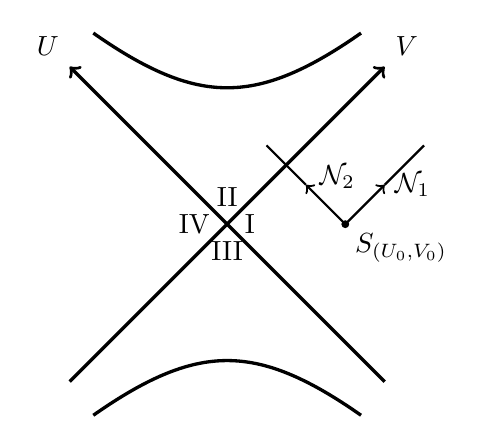
\begin{tikzpicture}
            \draw[domain=-1.7:1.7,smooth,variable=\x,very thick] plot({\x},{sqrt(3+\x*\x))});
            \draw[domain=-1.7:1.7,smooth,variable=\x,very thick] plot({\x},{-sqrt(3+\x*\x))});
            \draw[very thick,->] (-2,-2) -- (2,2) node[above right] {\(V\)};
            \draw[very thick,->] (2,-2) -- (-2,2) node[above left] {\(U\)};
            \draw (0.1,0) node[right] {I};
            \draw (0,0.1) node[above] {II};
            \draw (0,-0.1) node[below] {III};
            \draw (-0.1,0) node[left] {IV};
            
            \fill (1.5,0) circle (0.05) node[below right] {\(S_{(U_0,V_0)}\)};
            \draw[thick, ->] (1.5,0) -- (2,0.5) node[right] {\(\mathcal{N}_1\)};
            \draw[thick] (2,0.5) -- (2.5,1);
            \draw[thick, ->] (1.5,0) -- (1,0.5);
            \node[right] at (1.05,0.6) {\(\mathcal{N}_2\)};
            \draw[thick] (1,0.5) -- (0.5,1);
        \end{tikzpicture}
    \end{figure}
    Each null surface contains geodesic tangent vectors of the form \((\dd{U})^a\propto re^{\frac{r}{2M}}\left(\pdv{V}\right)^a = U_1^a\) and \((\dd{V})^a\propto re^{\frac{r}{2M}}\left(\pdv{U}\right)^a = U_2^a\) respectively. We have
    \begin{align}
        \theta_1 = \nabla_aU_1^a &= \frac{1}{\sqrt{-g}}\partial_\mu(\sqrt{-g}U_1^\mu) \\
                                 &= r^{-1}e^{\frac{r}{2M}}\partial_V(re^{-\frac{r}{2M}}re^{\frac{r}{2M}}) \\
                                 &= 2e^{\frac{r}{2M}} \partial_V r.
    \end{align}
    Using \(UV = -e^{\frac{r}{2M}}\left(\frac{r}{2M}-1\right)\) we can find \(\partial_V r\), and so can obtain \(\theta_1 = -\frac{8M^2}{r}U\). Similarly we have \(\theta_2 = -\frac{8M^2}{r}V\). We set \(U=U_0\) and \(V=V_0\) to find the expansion of the two surfaces.

    If \(\mathcal{S}\) is in region I, we have \(\theta_1>0\) and \(\theta_2<0\), so this is not a trapped surface. However, if \(\mathcal{S}\) is in the black hole region II, then \(\theta_1, \theta_2 < 0\), and so \(\mathcal{S}\) is trapped.
\end{eg}

\subsection{Raychaudhuri's equation}
\lecture{05/02/16}
\begin{lemma}
    \emph{Raychaudhuri's equation} holds:
    \begin{equation}
        \dv{\theta}{\lambda} = -\frac{1}{2}\theta^2 - \hat{\sigma}^{ab}\hat{\sigma}_{ab} + \hat{\omega}^{ab}\hat{\omega}_{ab} - R_{ab}U^aU^b
    \end{equation}
\end{lemma}
\begin{proof}
    We have 
    \begin{align}
        \dv{\theta}{\lambda} &= U\vdot\nabla(B\indices{^a_b}P\indices{^b_a}) = P\indices{^b_a}U\vdot\nabla B\indices{^a_b} \\
                             &= P\indices{^b_a}U^c\nabla_c\nabla_b U^a \\
                             &= P\indices{^b_a}U^c(\nabla_b\nabla_c U^a + R\indices{^a_{dcb}}U^d) \\
                             &= P\indices{^b_a}(\nabla_b(\underbrace{U^c\nabla_cU^a}_{=0}) - (\nabla_bU^c)\nabla_cU^a) + P\indices{^b_a} R\indices{^a_{dcb}}U^cU^d \\
                             &= - B\indices{^c_b}P\indices{^b_a}B\indices{^a_c} - R_{cd} U^cU^d \\
                             &= -\hat{B}\indices{^c_a}\hat{B}\indices{^a_c} - R_{ab}U^aU^b \\
                             &= -\frac{1}{2}\theta^2 - \hat{\sigma}^{ab}\hat{\sigma}_{ab} + \hat{\omega}^{ab}\hat{\omega}_{ab} - R_{ab}U^aU^b.
    \end{align}
\end{proof}

\subsection{Conditions on energy}
Often we will impose energy conditions on the energy momentum tensor.

\subsubsection*{Dominant energy condition}
This states that \(-T\indices{^a_b}V^b\) is a future-directed causal vector (or zero) for all future-directed timelike vectors \(V\). The DEC implies that if \(T_{ab} = 0\) in a closed \(\mathcal{S} \in \Sigma\), then \(T_{ab} = 0\) in \(D^+(\mathcal{S})\). Said another way: nothing can travel faster than the speed of light.

\begin{eg}
    Consider the energy-momentum tensor of a scalar field
    \begin{equation}
        T_{ab} = \partial_a\phi\partial_b\phi - \frac{1}{2}g_{ab}(\partial\phi)^2.
    \end{equation}
    We define \(j^a = -T\indices{^a_b}V^b\). We have
    \begin{equation}
        j^a = -(V\vdot\partial\phi)\partial^a\phi + \frac{1}{2}V^a(\partial\phi)^2 
        \implies
        j^2 = \frac{1}{4}\underbrace{V^2}_{<0}\underbrace{\left((\partial\phi)^2\right)^2}_{\ge 0} 
        \le 0,
    \end{equation}
    so \(j\) is causal or zero. Also
    \begin{equation}
        V\vdot j = -(V\vdot\partial\phi)^2 + \frac{1}{2}V^2(\partial\phi)^2 = \underbrace{-\frac{1}{2}(V\vdot\partial\phi)^2}_{\le 0} + \underbrace{\frac{1}{2}V^2}_{<0} \underbrace{\left[\partial\phi - \frac{V\vdot\partial\phi}{V^2}V\right]^2}_{\perp V^a \implies \ge 0} \le 0,
    \end{equation}
    so \(j\) is future-directed. Therefore scalar fields obey the DEC.
\end{eg}

\subsubsection*{Weak energy condition}
This states that \(T_{ab}V^aV^b\ge 0\) for all causal vectors \(V^a\). Note that DEC \(\implies\) WEC.

\subsubsection*{Null energy condition}
This states that \(T_{ab}V^aV^b\ge 0\) for all \emph{null} vectors \(V^a\). Note that WEC \(\implies\) NEC.

\subsubsection*{Strong energy condition}
This states that \((T_{ab}-\frac{1}{2}g_{ab}T\indices{^c_c})V^aV^b \ge 0\) for all causal vectors \(V^a\). Alternatively, using Einstein's equations, \(R_{ab}V^aV^b\ge0\), i.e.\ ``gravity is attractive''.

The SEC is independent to the other three; it is neither implied by, nor does it imply, any of the DEC, WEC or NEC.

\end{document}
